% RCR-YOLO 论文 LaTeX 源文件（中文版）
% 编译：XeLaTeX
% 模板：IEEE Transactions

\documentclass[journal]{IEEEtran}

% 中文支持
\usepackage{xeCJK}
\setCJKmainfont{SimSun} % 宋体

% 基础包
\usepackage{cite}
\usepackage{amsmath,amssymb,amsfonts}
\usepackage{algorithmic}
\usepackage{graphicx}
\usepackage{textcomp}
\usepackage{xcolor}
\usepackage{booktabs}

% 超链接
\usepackage{hyperref}
\hypersetup{
    colorlinks=true,
    linkcolor=blue,
    filecolor=magenta,
    urlcolor=cyan,
}

% 文档信息
\title{RCR-YOLO：面向室内环境的鲁棒上下文感知区域检测}

\author{作者姓名待补充}

\begin{document}

\maketitle

% ==================== 摘要 ====================
\begin{abstract}
室内物体检测面临小尺度、遮挡和拥挤等挑战，这些挑战会降低通用检测器的性能。我们提出RCR-YOLO，一种基于YOLO11n的鲁棒检测方法，包含三个互补模块。ORB-In通过物体区域和边界重建提供训练时的辅助监督，在零推理开销下增强小目标特征学习。MRFE采用多感受野机制，通过并行膨胀卷积和动态加权改善多尺度表示。LCRBase通过多尺度池化集成轻量级场景级上下文，简化完整上下文推理以实现稳定的单阶段集成。在COCO-indoor上的系统消融实验验证了各组件的贡献和协同效应。我们的方法达到0.3433 mAP50-95（相比基线+3.7\%）和0.3343 Hard AP50-95（+3.8\%），在小目标、遮挡和拥挤场景上均有一致改进。三种子验证展示卓越稳定性（AP50-95标准差±0.0005 vs 基线±0.0012）。部署模型需要3.17M参数，RTX 4090上延迟10.36ms，保持实时性能（约96 FPS）。结果表明将两阶段上下文机制有效适配到单阶段检测框架用于室内环境。
\end{abstract}

\begin{IEEEkeywords}
物体检测，室内环境，多感受野，上下文推理，YOLO，服务机器人
\end{IEEEkeywords}

% ==================== 第I节：引言 ====================
\section{引言}
\label{sec:introduction}

\subsection{动机与背景}
\label{subsec:motivation}

室内服务机器人在家庭辅助、医疗护理、智能仓储和养老设施等应用中日益普及\cite{service_robot1,service_robot2}。可靠的物体检测是自主导航、人机交互和任务执行的基础能力。然而，室内环境呈现出独特的挑战，使其与现有文献中常见的户外或通用检测场景显著不同。

室内场景中，物体尺度分布偏向小型桌面物品（杯子、遥控器、手机、键盘等），这些目标在特征图中仅占据几个像素，容易被背景杂波淹没。遮挡无处不在——家具、人体和物体间的相互遮挡导致目标部分可见、边界模糊，需要鲁棒的空间推理能力推断完整物体形状。场景拥挤是另一普遍特征——书架、桌面和厨房台面常出现密集排列的物体，边界框严重重叠，丰富的上下文信息难以有效利用。这些挑战在服务机器人的典型工作环境中交织出现，对检测系统提出了严峻考验。

现有通用检测器如YOLO系列\cite{redmon2016yolo,bochkovskiy2020yolov4,ultralytics2023yolov8}和R-CNN家族\cite{girshick2014rcnn,ren2015faster}在大规模数据集（如MS COCO\cite{lin2014microsoft}）上取得了令人印象深刻的结果。然而，这些方法针对所有COCO类别的平衡性能进行优化，在室内特定场景下表现退化。局限性包括：(1)对底层特征学习的监督不足——标准检测损失仅在正样本锚点位置施加约束，对小目标的空间分布和轮廓学习引导较弱；(2)有限的多尺度表示能力——固定感受野的卷积难以适应从几像素到数百像素的极端尺度变化；(3)上下文信息利用不足——通用检测器缺乏针对室内遮挡和拥挤场景的显式上下文推理机制。针对室内场景的专门设计仍然不足。

受重建任务在表示学习中的成功、多感受野机制在多尺度检测中的有效性、以及上下文推理在困难场景中的潜力启发，我们提出RCR-YOLO，一种面向室内环境的鲁棒上下文感知检测方法。基于轻量级的YOLO11n架构，我们设计三个互补模块：ORB-In通过训练时的物体区域和边界重建提供辅助监督，在零推理开销下增强小目标底层特征学习；MRFE采用多感受野机制，通过并行膨胀卷积和动态加权改善多尺度表示；LCRBase通过多尺度池化集成轻量级场景级上下文，简化完整上下文推理以实现稳定的单阶段集成。系统消融实验在COCO-indoor数据集上验证了各组件的独立贡献和协同效应，三种子验证展示了方法的稳定性和可靠性。

\subsection{主要贡献}
\label{subsec:contributions}

本文的主要贡献总结如下：

\begin{enumerate}
    \item \textbf{RCR-YOLO架构}：我们提出一种针对室内环境的检测方法，通过三个互补模块（ORB-In、MRFE、LCRBase）协同增强YOLO11n，针对小目标、遮挡和拥挤等室内挑战提供专门设计。

    \item \textbf{训练-推理不对称设计}：ORB-In模块在训练时提供物体区域和边界重建监督，增强底层特征学习，推理时完全旁路实现零推理开销，平衡性能提升与实时性要求。

    \item \textbf{单阶段上下文推理适配}：LCRBase简化完整LCR的难度门控和区域聚合机制，仅保留场景级上下文增强，解决两阶段上下文推理方法在单阶段检测器中的不稳定性问题（三种子验证显示方差降低5倍）。

    \item \textbf{系统评估与验证}：在COCO-indoor数据集上进行10配置消融实验，关键模型进行三种子验证，配对t检验证明改进的统计显著性（p<0.05），Hard v2协议评估困难场景性能，定性可视化展示实际改进效果。

    \item \textbf{实用性能}：ab4-rcr-fb配置达到0.3433 mAP50-95（相比baseline +3.7\%）和0.3343 Hard AP50-95（+3.8\%），在小目标、遮挡和拥挤场景上均有一致改进，同时保持实时性能（~96 FPS，3.17M参数，10.36ms延迟）。
\end{enumerate}

\subsection{论文组织}
\label{subsec:organization}

本文其余部分组织如下：第\ref{sec:related_work}节回顾相关工作，包括通用物体检测、室内检测方法、特征增强技术和上下文建模。第\ref{sec:methodology}节详细描述RCR-YOLO架构，包括ORB-In、MRFE和LCRBase三个模块的设计与实现。第\ref{sec:experiments}节展示COCO-indoor数据集上的实验结果，包括消融实验、基线对比、统计显著性验证、困难场景分析和效率评估。第\ref{sec:discussion}节讨论设计选择、模块协同效应和局限性。第\ref{sec:conclusion}节总结全文并展望未来工作方向。

% ==================== 第II节：相关工作 ====================
\section{相关工作}
\label{sec:related_work}

\subsection{通用物体检测}
\label{subsec:general_detection}

物体检测经历了从两阶段到单阶段再到基于Transformer方法的演进。\textbf{两阶段检测器}以R-CNN\cite{girshick2014rcnn}开创proposal-based范式，Fast R-CNN\cite{girshick2015fast}和Faster R-CNN\cite{ren2015faster}通过RoI pooling和Region Proposal Network（RPN）提升效率。Cascade R-CNN\cite{cai2018cascade}引入级联精炼，逐步提高定位质量。两阶段方法在精度上表现优异，但推理延迟较高（通常>50ms），限制了实时应用。

\textbf{单阶段检测器}直接在密集特征图上预测，大幅降低延迟。YOLO系列\cite{redmon2016yolo,redmon2017yolo9000,bochkovskiy2020yolov4}持续演化：YOLOv3引入多尺度检测和FPN结构，YOLOv5通过工程优化和部署友好设计获得广泛应用，YOLOv8\cite{ultralytics2023yolov8}引入C2f模块和改进的损失函数，YOLOv10\cite{wang2024yolov10}提出端到端检测消除NMS后处理，YOLO11\cite{ultralytics2023yolo11}采用C3k2和C2PSA模块进一步提升性能。SSD\cite{liu2016ssd}使用多尺度特征图，RetinaNet\cite{lin2017focal}提出Focal Loss解决类别不平衡。单阶段方法在速度-精度权衡上表现出色，但在小目标和拥挤场景的性能仍有提升空间。

\textbf{基于Transformer的检测器}近年兴起。DETR\cite{carion2020detr}引入端到端Transformer架构，Deformable DETR\cite{zhu2020deformable}通过可变形注意力提升效率和小目标性能。然而，Transformer方法训练成本高、收敛慢，在资源受限场景的实用性有限。

通用检测器在大规模数据集（如COCO\cite{lin2014microsoft}）上取得优异性能，但在专门的室内场景仍存在性能差距。本文基于单阶段YOLO框架，针对室内挑战进行专门增强。

\subsection{室内物体检测}
\label{subsec:indoor_detection}

室内环境具有独特特点：尺度分布偏向小目标（桌面物品占比高）、普遍遮挡（家具和物体间相互遮挡）、类别分布不平衡（少数家具类别与众多小物品类别）、光照和视角变化多样（室内照明条件复杂，机器人视角多变）。这些特点使得通用检测器在室内场景表现受限。

近期工作针对室内挑战进行探索。文献\cite{chen2020enhanced}提出改进的SSD变体，针对室内小目标设计多尺度特征融合策略。文献\cite{zhang2021indoor}引入多尺度注意力机制用于室内检测，通过自适应特征加权提升小目标和遮挡目标性能。然而，现有室内检测方法大多采用相对简单的特征增强策略，对上下文信息的利用不足，训练监督可通过辅助任务进一步丰富。

值得注意的是，文献\cite{chen2020enhanced,zhang2021indoor}未提供公开实现，论文中缺少足够的实现细节（网络架构具体参数、训练超参数、数据预处理流程）以进行忠实复现。这限制了我们进行直接对比，本文主要与YOLO系列基线对比，并在局限性部分讨论领域专门方法对比的缺失。

本文提出的RCR-YOLO通过三个模块协同设计，系统地应对室内检测的小目标、遮挡和拥挤挑战，在单阶段框架中实现有效的上下文推理增强。

\subsection{特征增强方法}
\label{subsec:feature_enhancement}

有效的特征表示是检测性能的基础。\textbf{多尺度特征融合}架构如FPN\cite{lin2017fpn}、PANet\cite{liu2018path}和BiFPN\cite{tan2020efficientdet}通过自顶向下和自底向上路径聚合不同层级特征，改善多尺度目标检测。YOLO系列广泛采用这些特征金字塔设计。

\textbf{注意力机制}显式建模通道和空间重要性。SE\cite{hu2018squeeze}通过全局池化和全连接层生成通道注意力权重，CBAM\cite{woo2018cbam}结合通道和空间注意力，ECA\cite{wang2020eca}通过一维卷积实现高效通道注意力。这些机制在分类和检测任务中广泛应用。

\textbf{多感受野设计}通过并行分支捕获不同范围的上下文。ORFENet\cite{orfe2021}提出多感受野自适应特征增强，使用不同膨胀率的并行分支和动态权重融合，在小目标检测上展现优势。Inception系列\cite{szegedy2015going}通过多尺度卷积核并行提取多粒度特征。YOLO-SM\cite{yolosm2022}提供轻量级卷积实现参考。

我们的MRFE模块受ORFENet启发，但进行单阶段适配：(1)使用深度可分离卷积减少参数量约60\%，满足实时性约束；(2)采用轻量级GAP+1$\times$1卷积生成动态权重，而非复杂的多头注意力；(3)在固定Neck尺度（P3/16, P4/32, P5/64）插入，保持YOLO架构完整性。这些适配使MRFE更适合资源受限的机器人部署场景。

\subsection{上下文建模}
\label{subsec:context_modeling}

困难目标（小尺度、遮挡、拥挤）需要更丰富的上下文线索。\textbf{全局上下文方法}如Non-local Neural Networks\cite{wang2018non}通过自注意力机制建模全局依赖，GCNet\cite{cao2019gcnet}简化Non-local为全局上下文块，减少计算开销。这些方法在分类和分割任务中有效，但在检测中的应用受限于计算成本。

\textbf{区域关系建模}显式利用物体间关系。CRNet\cite{chi2020crnet}引入易-帮-难（easy-help-hard）机制，易检测区域通过上下文推理辅助困难区域检测。IENet\cite{hu2021ienet}建模区域级交互用于实例级理解，通过区域特征聚合增强遮挡目标检测。这些方法在两阶段检测器（Faster R-CNN）中展示强性能，利用显式proposal区域定义易/难分区和区域关系。

然而，\textbf{将两阶段上下文推理方法直接迁移到单阶段YOLO面临挑战}：(1)无proposal阶段——单阶段检测器直接在密集特征图上操作，缺少显式区域建议，易/难分区不可行；(2)基于特征图的难度估计不稳定——缺少proposal引导的难度估计在密集预测中方差大；(3)区域选择和聚合机制增加计算开销，复杂化实时部署。

我们的LCRBase模块简化完整LCR（轻量级上下文推理），移除难度门控和易区域聚合，仅保留场景级全局上下文增强。多尺度池化（1$\times$1, 2$\times$2, 4$\times$4）捕获全局和半全局上下文，轻量级1$\times$1卷积融合特征。这种简化设计在单阶段框架中实现稳定集成，三种子验证显示方差降低5倍（LCRBase std ±0.0020 vs 完整LCR std ±0.0102），同时保持上下文推理的有效性。

本文的工作受上述方法启发，但针对室内单阶段检测进行系统适配。ORB-In的训练-推理不对称设计借鉴重建任务在表示学习中的成功，MRFE将多感受野机制轻量化并集成到YOLO Neck，LCRBase将两阶段上下文推理简化为场景级增强以适配单阶段框架。三模块协同设计形成针对室内挑战的完整解决方案。


% ==================== 第III节：方法 ====================
\section{方法}
\label{sec:methodology}

\subsection{整体架构}
\label{subsec:overall_architecture}

图\ref{fig:architecture}展示了RCR-YOLO的整体架构。输入的RGB图像（640$\times$640）通过YOLO11n骨干网络（CSPDarknet变体）提取多层级特征$\{P_2, P_3, P_4, P_5\}$。骨干网络基于跨阶段局部网络（CSP）设计，通过多个C3k2模块和C2PSA（跨阶段局部注意力）模块进行特征提取，生成不同尺度的特征金字塔。

\textbf{特征提取流程：}输入图像首先经过初始卷积层进行下采样，随后通过四个阶段的特征提取，每个阶段将特征图分辨率减半同时增加通道数。对于640$\times$640的输入：
\begin{itemize}
    \item $P_2$：160$\times$160分辨率，用于检测小目标
    \item $P_3$：80$\times$80分辨率，对应检测头P3/16
    \item $P_4$：40$\times$40分辨率，对应检测头P4/32
    \item $P_5$：20$\times$20分辨率，对应检测头P5/64
\end{itemize}

\textbf{ORB-In模块}作用于$P_2$特征层，在训练期间生成辅助重建监督。该模块将$P_2$特征（C$\times$160$\times$160）上采样至320$\times$320，通过卷积层输出双通道预测：通道0编码物体区域掩码，通道1编码边缘图。重建监督直接源自检测框标注，无需额外人工标注。关键设计在于推理时完全旁路该分支，因此部署模型中不包含ORB-In参数，实现零推理成本。

\textbf{Neck特征融合}遵循YOLO11n原生设计，采用PANet风格的自底向上和自顶向下路径聚合网络。Neck包含多个C3k2和C2PSA模块，实现不同尺度特征的有效融合。自底向上路径将深层语义信息传播到浅层，自顶向下路径将浅层细节信息传播到深层，形成丰富的多尺度特征表示。

\textbf{MRFE模块}插入三个检测尺度$\{P_3/16, P_4/32, P_5/64\}$，位于Neck特征融合之后、检测头之前。每个尺度独立应用一个MRFE实例，参数不共享。MRFE通过三个并行的膨胀深度可分离卷积分支（膨胀率d$\in\{1,2,3\}$）提取不同范围的上下文，并通过动态加权机制自适应融合。插入位置的选择确保不干扰Neck的特征传播路径，同时增强检测头的输入特征。

\textbf{LCRBase模块}在检测头前应用，对三个检测尺度并行增强场景级上下文。LCRBase通过多尺度自适应平均池化（1$\times$1，2$\times$2，4$\times$4）捕获全局、半全局和局部-全局上下文，经卷积融合后通过残差连接增强原始特征。与完整的LCR（轻量级上下文推理）不同，LCRBase移除了难度门控和易检测区域聚合机制，简化设计以适配单阶段检测器。

\textbf{检测头}采用YOLO11n的Detect Head，对每个尺度的特征进行类别概率预测和边界框回归。检测头包含分类分支和定位分支，分类分支输出各类别的置信度，定位分支预测边界框的中心坐标、宽高以及分布焦点损失（DFL）的分布参数，实现精细化定位。

\textbf{训练与推理的差异}是本架构的重要特点。训练阶段，ORB-In分支参与损失计算，通过梯度反传增强骨干网络底层特征学习，模型总参数包括检测器参数加0.075M的ORB-In参数。推理阶段，ORB-In分支完全旁路，部署模型仅包含检测器参数（MRFE和LCRBase保留），因此GFLOPs和推理延迟不受ORB-In影响。这种设计在训练时提供额外监督信号，同时满足服务机器人对实时性（$<$15ms）的严格要求。

\textbf{信息流概览}：输入图像 $\rightarrow$ 骨干网络特征提取 $\rightarrow$ ORB-In训练监督（P2层）$\rightarrow$ Neck特征融合 $\rightarrow$ MRFE多感受野增强 $\rightarrow$ LCRBase上下文增强 $\rightarrow$ 检测头输出 $\rightarrow$ 类别+边界框。整个流程保持端到端可微，所有模块通过联合优化共同训练。


\subsection{ORB-In：物体区域与边界重建}
\label{subsec:orb_in}

\subsubsection{动机}

室内场景中的小目标在特征图中占据像素数极少，容易被背景杂波淹没。标准检测损失仅在正样本锚点位置施加监督，对底层特征学习的约束不足。受重建任务在表示学习中成功的启发，我们提出通过训练时的物体区域和边界重建提供辅助监督，显式引导网络学习空间分布和轮廓信息，从而增强小目标特征表示。该分支在推理时旁路，不增加部署成本。

\textbf{与ORFENet的区别：}ORFENet采用物体级重建并依赖实例分割标签，而我们的ORB-In使用基于检测框的代理监督，无需额外标注。ORFENet的重建分支在推理时参与特征精炼，而ORB-In在部署时旁路以实现零推理开销。这一设计选择优先考虑机器人应用中至关重要的实时性能。

\subsubsection{模块设计}

ORB-In模块的输入为$P_2$特征（C$\times$H/4$\times$W/4），对于640$\times$640输入，$P_2$分辨率为C$\times$160$\times$160。架构流程如下：

\begin{enumerate}
    \item \textbf{上采样}：对$P_2$特征进行2$\times$双线性上采样至320$\times$320，恢复空间分辨率以实现像素级预测
    \item \textbf{特征变换}：3$\times$3卷积 + 批归一化（BN）+ SiLU激活
    \item \textbf{输出映射}：1$\times$1卷积生成2通道输出
    \begin{itemize}
        \item 通道0：物体区域掩码（二值，0表示背景，1表示前景）
        \item 通道1：边缘图（二值，0表示非边缘，1表示边缘）
    \end{itemize}
\end{enumerate}

\textbf{监督目标生成：}给定检测框标注$\{(x, y, w, h, \text{class})\}$，监督目标生成过程为：
\begin{itemize}
    \item \textit{区域掩码}：将每个检测框区域填充为1，背景区域为0，生成尺寸为320$\times$320的二值掩码$M_{\text{region}}$
    \item \textit{边缘图}：对区域掩码$M_{\text{region}}$应用Canny边缘检测或形态学梯度操作（膨胀-腐蚀），提取物体边界，生成尺寸为320$\times$320的二值边缘图$M_{\text{edge}}$
\end{itemize}

\textbf{损失函数}定义为：
\begin{equation}
\mathcal{L}_{\text{ORB}} = \mathcal{L}_{\text{region}} + \lambda_{\text{edge}} \cdot \mathcal{L}_{\text{edge}}
\end{equation}
其中$\mathcal{L}_{\text{region}}$和$\mathcal{L}_{\text{edge}}$均为二值交叉熵损失（BCE Loss），$\lambda_{\text{edge}}=1.0$。具体形式为：
\begin{equation}
\mathcal{L}_{\text{region}} = -\frac{1}{N}\sum_{i=1}^{N}\left[M_i^{\text{gt}}\log(\hat{M}_i) + (1-M_i^{\text{gt}})\log(1-\hat{M}_i)\right]
\end{equation}
其中$N=320\times 320$为像素总数，$M_i^{\text{gt}}$为真值掩码，$\hat{M}_i$为预测概率。$\mathcal{L}_{\text{edge}}$形式相同，作用于边缘预测。

重建目标直接对应检测框标注，无需额外的像素级或实例级标注，保持训练数据需求与标准检测相同。

\textbf{参数量}：ORB-In模块约0.075M参数，仅在训练时存在。

\subsubsection{训练与推理}

\textbf{训练阶段}，ORB-In分支参与损失计算，总损失函数为：
\begin{equation}
\mathcal{L}_{\text{total}} = \mathcal{L}_{\text{det}} + \lambda_{\text{ORB}} \cdot \mathcal{L}_{\text{ORB}}
\end{equation}
其中$\mathcal{L}_{\text{det}}$为检测损失（将在第\ref{subsec:loss_function}节详述），$\lambda_{\text{ORB}}=1.0$。ORB-In分支通过梯度反传增强骨干网络底层特征学习，使网络在提取特征时更关注物体区域和边界信息。

\textbf{推理阶段}，ORB-In分支完全旁路，相应参数不加载到部署模型。因此：
\begin{itemize}
    \item 训练参数 = 检测器参数 + 0.075M（ORB-In）
    \item 部署参数 = 检测器参数（仅）
    \item 推理GFLOPs和延迟不受影响
\end{itemize}

\textbf{设计理由}：训练时提供额外监督信号，通过像素级重建任务增强小目标特征表示，特别是增强对小目标空间位置和形状轮廓的感知能力。推理时零成本设计满足服务机器人实时性要求（$<$15ms延迟预算）。这种训练-推理不对称设计在保证性能提升的同时避免了推理开销，是针对资源受限部署场景的实用权衡。


\subsection{MRFE：多感受野特征增强}
\label{subsec:mrfe}

\subsubsection{动机}

室内物体在尺度上跨度大，从小型桌面物品（几个像素）到大型家具（数百像素）。单一感受野的卷积在捕获这种尺度变化时受限：小感受野关注局部细节但缺乏上下文，大感受野提供上下文但可能模糊小目标边界。受ORFENet多感受野机制成功的启发，我们提出MRFE通过并行的多尺度感受野增强检测特征表示，使网络能够同时捕获局部细节、中等范围和大范围上下文。

\textbf{与ORFENet的适配：}我们采用ORFENet的多感受野概念，但为YOLO集成进行简化。关键差异：(1)我们使用深度可分离卷积代替标准卷积，参数量减少约60\%以满足实时性约束；(2)我们的动态加权采用轻量级全局平均池化和1$\times$1卷积，而非复杂的多头注意力模块；(3)我们在三个固定的Neck尺度（P3/16, P4/32, P5/64）插入MRFE，而非可学习的自适应特征金字塔，保持YOLO架构完整性并避免额外的金字塔构建开销。

\subsubsection{模块设计}

MRFE模块的输入特征$\mathbf{X} \in \mathbb{R}^{C \times H \times W}$通过三个并行分支处理，每个分支采用不同膨胀率的深度可分离卷积：

\textbf{分支设计：}
\begin{equation}
\mathbf{F}_d = \text{DWSConv}(\mathbf{X}, d), \quad d \in \{1, 2, 3\}
\end{equation}
其中DWSConv为深度可分离卷积，定义为：
\begin{equation}
\text{DWSConv}(\mathbf{X}, d) = \text{Conv}_{1\times1}(\text{DepthConv}_{3\times3}(\mathbf{X}, d))
\end{equation}
$\text{DepthConv}_{3\times3}(\mathbf{X}, d)$表示膨胀率为$d$的3$\times$3深度卷积，每个输入通道独立进行卷积；$\text{Conv}_{1\times1}$为逐点卷积，将通道间信息混合。每个分支后接批归一化（BN）和SiLU激活函数，产生特征$\{\mathbf{F}_1, \mathbf{F}_2, \mathbf{F}_3\}$。

\textbf{感受野语义：}
\begin{itemize}
    \item $d=1$（无膨胀）：标准3$\times$3感受野，捕获局部细节、纹理和边缘
    \item $d=2$（膨胀2）：有效感受野5$\times$5，捕获中等范围上下文和物体中心区域
    \item $d=3$（膨胀3）：有效感受野7$\times$7，捕获大范围上下文、物体完整轮廓和相邻物体关系
\end{itemize}

\textbf{动态权重生成：}三个分支的特征首先拼接，随后通过全局平均池化和1$\times$1卷积生成动态权重：
\begin{equation}
\mathbf{F}_{\text{cat}} = \text{Concat}(\mathbf{F}_1, \mathbf{F}_2, \mathbf{F}_3) \in \mathbb{R}^{3C \times H \times W}
\end{equation}
\begin{equation}
\mathbf{g} = \text{GAP}(\mathbf{F}_{\text{cat}}) \in \mathbb{R}^{3C \times 1 \times 1}
\end{equation}
\begin{equation}
\mathbf{w} = \sigma(\text{Conv}_{1\times1}(\mathbf{g})) \in \mathbb{R}^{3C \times 1 \times 1}
\end{equation}
其中GAP表示全局平均池化，$\sigma$为Sigmoid激活函数。权重向量$\mathbf{w}$被分割为三个部分$\{\mathbf{w}_1, \mathbf{w}_2, \mathbf{w}_3\}$，每部分$\mathbf{w}_d \in \mathbb{R}^{C \times 1 \times 1}$对应一个膨胀率分支。

\textbf{加权融合：}最终输出通过加权求和和残差连接生成：
\begin{equation}
\mathbf{Y} = \mathbf{X} + \sum_{d=1}^{3} (\mathbf{w}_d \odot \mathbf{F}_d)
\end{equation}
其中$\odot$表示逐通道加权（通道维度广播相乘）。残差连接$\mathbf{X}$保留原始信息，稳定训练并防止梯度消失。

\textbf{设计理由：}
\begin{itemize}
    \item \textit{深度可分离卷积}：标准3$\times$3卷积参数量为$C \times C \times 3 \times 3$，深度可分离卷积参数量为$C \times 3 \times 3 + C \times C \times 1 \times 1$，当$C$较大时参数减少约$(9C^2) / (9C + C^2) \approx 60\%$
    \item \textit{动态权重}：不同场景和位置需要不同的感受野组合，动态权重实现自适应选择。例如，小目标区域$d=1$权重高，大目标和遮挡区域$d=3$权重高
    \item \textit{残差连接}：保持原始特征，确保即使动态权重学习不充分，网络性能也不会退化
\end{itemize}

\subsubsection{Neck集成}

MRFE模块插入YOLO11n Neck的三个检测尺度，位于特征融合后、检测头前：
\begin{itemize}
    \item \textbf{P3/16尺度}（80$\times$80 for 640输入）：针对小到中等尺度目标（16-64像素）
    \item \textbf{P4/32尺度}（40$\times$40）：针对中到大尺度目标（32-128像素）
    \item \textbf{P5/64尺度}（20$\times$20）：针对大尺度目标（64像素以上）
\end{itemize}

每个尺度独立应用一个MRFE实例，参数不共享。这种设计允许每个尺度学习适合其目标尺寸范围的感受野组合。插入位置选择在Neck的自底向上和自顶向下路径完成后，避免干扰特征金字塔的传播动态，同时直接增强送入检测头的特征。

\textbf{参数分配：}假设三个检测尺度的通道数分别为$\{C_3, C_4, C_5\}$（YOLO11n中典型值为$\{128, 256, 512\}$），每个MRFE实例的参数量约为：
\begin{equation}
\begin{split}
\text{Params}_{\text{MRFE}} &\approx 3 \times (C \times 3 \times 3 + C \times C) \\
&\approx 3 \times C \times (9 + C)
\end{split}
\end{equation}
对于$C=256$（P4尺度），单个MRFE约0.20M参数。三个尺度总计约0.25M参数。

\textbf{推理开销：}单个MRFE模块约增加0.9ms延迟（RTX 4090, FP32, batch=1），三个尺度总计增加约2.75ms。开销主要来自三个并行深度可分离卷积分支和动态权重计算。尽管如此，总延迟仍保持在实时范围内（详见表\ref{tab:efficiency}）。

\textbf{与单一感受野的对比：}标准YOLO11n在每个检测尺度使用固定的卷积操作，感受野范围有限。MRFE通过并行多膨胀率卷积和自适应加权，显著扩展了有效感受野范围，使网络能够同时捕获多尺度信息。消融实验（表\ref{tab:ablation}）显示，MRFE单独提供最大的单模块增益（mAP50-95 +0.0058），验证多感受野机制对多尺度目标检测的有效性。


\subsection{LCRBase：轻量级上下文推理}
\label{subsec:lcrbase}

\subsubsection{动机}

困难目标（小尺度、遮挡、拥挤）需要更丰富的上下文线索。CRNet提出易-帮-难机制，利用易检测区域辅助困难区域。IENet建模区域间关系。这些方法在两阶段检测器中展示强性能，但直接迁移到单阶段YOLO面临挑战：缺少proposal阶段使得显式易/难区域区分困难。我们提出LCRBase，通过简化上下文推理机制，仅保留场景级上下文增强，避免复杂的难度门控和区域聚合，实现轻量级上下文推理在单阶段框架中的稳定集成。

\textbf{单阶段适配挑战：}CRNet和IENet依赖两阶段检测器的显式proposal区域定义易/难分区。直接迁移到单阶段YOLO失败的原因：(1)无proposal阶段——单阶段检测器直接在密集特征图上操作，没有区域建议，显式易/难分区不可行；(2)基于特征图的难度估计不稳定，缺少proposal引导——我们的三种子消融验证了这一点，显示包含完整LCR的rcr-full在拥挤场景表现高方差（std ±0.0102 vs LCRBase ±0.0020）；(3)易区域筛选需要额外计算开销和区域选择机制，复杂化实时部署。我们的LCRBase通过多尺度池化仅保留场景级全局上下文，消除难度门控和区域选择，实现稳定的单阶段集成同时保持有效性。

\subsubsection{模块设计}

LCRBase模块的输入特征$\mathbf{X} \in \mathbb{R}^{C \times H \times W}$通过多尺度自适应平均池化提取场景上下文：

\textbf{多尺度池化：}
\begin{equation}
\begin{split}
\mathbf{P}_{1 \times 1} &= \text{AdaptiveAvgPool}_{1 \times 1}(\mathbf{X}) \in \mathbb{R}^{C \times 1 \times 1} \\
\mathbf{P}_{2 \times 2} &= \text{AdaptiveAvgPool}_{2 \times 2}(\mathbf{X}) \in \mathbb{R}^{C \times 2 \times 2} \\
\mathbf{P}_{4 \times 4} &= \text{AdaptiveAvgPool}_{4 \times 4}(\mathbf{X}) \in \mathbb{R}^{C \times 4 \times 4}
\end{split}
\end{equation}

每个池化尺度捕获不同范围的场景信息：
\begin{itemize}
    \item $1 \times 1$池化：全局上下文，整个场景的统计摘要
    \item $2 \times 2$池化：半全局上下文，场景的四个象限信息
    \item $4 \times 4$池化：局部-全局上下文，场景16个区域的粗粒度空间布局
\end{itemize}

\textbf{特征融合：}每个池化特征经1$\times$1卷积降维并上采样至原始尺寸$H \times W$，随后拼接：
\begin{equation}
\begin{split}
\mathbf{P}'_{s \times s} &= \text{Upsample}(\text{Conv}_{1 \times 1}(\mathbf{P}_{s \times s}), (H, W)) \\
\mathbf{C} &= \text{Concat}(\mathbf{P}'_{1 \times 1}, \mathbf{P}'_{2 \times 2}, \mathbf{P}'_{4 \times 4})
\end{split}
\end{equation}
其中Upsample为双线性插值上采样，Concat在通道维度拼接。拼接后的特征$\mathbf{C} \in \mathbb{R}^{3C' \times H \times W}$（其中$C'$为降维后通道数）经过一个1$\times$1卷积融合：
\begin{equation}
\mathbf{Y} = \mathbf{X} + \text{Conv}_{1 \times 1}(\mathbf{C})
\end{equation}
残差连接保留原始特征，上下文信息作为增强项添加。

\textbf{与完整LCR的差异：}
\begin{enumerate}
    \item \textit{不使用难度门控}：完整LCR基于特征图响应估计目标难度，在单阶段检测中此估计不稳定。三种子实验显示，rcr-full（包含完整LCR）在拥挤场景（crowd-heavy）标准差为±0.0102，而LCRBase标准差仅为±0.0020，方差降低5倍（表\ref{tab:three_seed}）。

    \item \textit{不使用易检测区域聚合}：完整LCR筛选易检测区域作为上下文源，辅助困难区域检测。LCRBase直接使用全局场景上下文，简化计算，避免区域选择机制引入的额外开销和不稳定性。

    \item \textit{仅保留场景级上下文}：多尺度池化捕获不同范围场景信息，轻量级1$\times$1卷积整合特征。这种简化设计在保持上下文推理有效性的同时，适配单阶段检测器的密集预测范式。
\end{enumerate}

\textbf{参数量与效率：}每个LCRBase实例约0.11M参数（假设$C'=C/2$降维）。三个检测尺度总计约0.32M参数。单个实例增加约0.3ms延迟，三个尺度总计约0.91ms（RTX 4090）。相比完整LCR，LCRBase参数量减少约40\%，延迟减少约30\%。

\subsubsection{与检测头连接}

LCRBase在检测头前并行应用于三个检测尺度$\{P_3, P_4, P_5\}$，每个尺度独立实例，参数不共享。增强后的特征直接送入YOLO11n的Detect Head进行类别预测和边界框回归。

\textbf{上下文信息隐式辅助检测：}
\begin{itemize}
    \item \textit{前景/背景区分}：全局场景上下文提供判别线索，辅助区分真实物体与背景杂波
    \item \textit{遮挡物体定位}：大范围上下文（$1 \times 1$和$2 \times 2$池化）捕获部分可见物体的完整空间布局，辅助推断被遮挡物体的完整轮廓
    \item \textit{拥挤场景处理}：多尺度上下文（特别是$4 \times 4$池化的粗粒度空间布局）辅助密集目标的分离和定位
\end{itemize}

\textbf{实验验证：}表\ref{tab:ablation}显示，单独LCRBase（ab3b-lcrbase）在crowd-heavy场景提升有限（AP50 +0.0011相比baseline）。然而，与ORB-In和MRFE组合后（ab4-rcr-fb），crowd-heavy场景改进显著（AP50 +0.0107相比baseline），验证上下文推理模块与底层和中层增强模块的协同效应。完整的三模块组合使LCRBase能够在更强的特征基础上发挥作用，有效利用场景上下文信息。


\subsection{损失函数}
\label{subsec:loss_function}

总损失函数为：
\begin{equation}
\mathcal{L}_{\text{total}} = \mathcal{L}_{\text{det}} + \lambda_{\text{ORB}} \cdot \mathcal{L}_{\text{ORB}}
\end{equation}

\textbf{检测损失}$\mathcal{L}_{\text{det}}$（YOLO11n原生损失）：
\begin{equation}
\mathcal{L}_{\text{det}} = \lambda_{\text{cls}} \mathcal{L}_{\text{cls}} + \lambda_{\text{box}} \mathcal{L}_{\text{box}} + \lambda_{\text{dfl}} \mathcal{L}_{\text{dfl}}
\end{equation}
其中：
\begin{itemize}
    \item $\mathcal{L}_{\text{cls}}$：分类损失，采用Varifocal Loss或二值交叉熵（BCE）
    \item $\mathcal{L}_{\text{box}}$：边界框损失，采用CIoU Loss（Complete Intersection over Union）
    \item $\mathcal{L}_{\text{dfl}}$：分布焦点损失（Distribution Focal Loss），用于精细化边界框预测
    \item $\lambda_{\text{cls}}$, $\lambda_{\text{box}}$, $\lambda_{\text{dfl}}$：YOLO11n默认权重
\end{itemize}

\textbf{ORB重建损失}$\mathcal{L}_{\text{ORB}}$（仅训练时）：
\begin{equation}
\mathcal{L}_{\text{ORB}} = \mathcal{L}_{\text{region}} + \lambda_{\text{edge}} \cdot \mathcal{L}_{\text{edge}}
\end{equation}
其中$\mathcal{L}_{\text{region}}$和$\mathcal{L}_{\text{edge}}$均为二值交叉熵损失，$\lambda_{\text{edge}}=1.0$。

\textbf{超参数设置：}
\begin{itemize}
    \item $\lambda_{\text{ORB}} = 1.0$（通过预备实验确定）
    \item 训练轮数：300 epochs
    \item Early stopping patience：50 epochs
    \item close\_mosaic：15（最后15轮关闭Mosaic增强）
    \item 学习率：$\text{lr}_0=0.01$，余弦退火衰减
    \item 优化器：SGD（momentum=0.937, weight\_decay=0.0005）
    \item Batch size：64
    \item 输入尺寸：640$\times$640
\end{itemize}

\textbf{数据增强：}
\begin{itemize}
    \item Mosaic（前285轮）：四张图像拼接，丰富尺度和背景多样性
    \item MixUp：随机混合两张图像，增强鲁棒性
    \item HSV颜色抖动：色调、饱和度、明度随机扰动
    \item 随机翻转：水平翻转概率0.5
\end{itemize}

训练模式为非确定性（cuDNN autotune启用），利用GPU算子自动调优提升训练速度。所有消融实验和基线对比使用相同的训练协议，确保公平比较。


% ==================== 第IV节：实验 ====================
\section{实验}
\label{sec:experiments}

\subsection{实验设置}
\label{subsec:experimental_setup}

\subsubsection{数据集}

我们使用COCO-indoor子集进行实验，该子集从MS COCO数据集\cite{lin2014microsoft}中提取室内相关类别。COCO数据集包含80个物体类别，其中约40-50个类别与室内场景相关，包括家具（沙发、椅子、桌子、床）、电子设备（电视、笔记本电脑、手机、键盘、鼠标）、厨房用品（碗、杯子、刀叉、微波炉、冰箱）、日常物品（书籍、时钟、花瓶、遥控器）等。我们使用标准的train/validation划分，训练集约118,000张图像，验证集约5,000张图像。

\textbf{Hard v2评估协议}用于更细粒度的困难场景分析。该协议将验证集实例按两个维度分桶：

\textit{尺寸桶}（基于边界框面积）：
\begin{itemize}
    \item Small（面积 $< 32^2$ 像素）：7,846个实例
    \item Medium（$32^2 \leq$ 面积 $< 96^2$）：9,431个实例
    \item Large（面积 $\geq 96^2$）：8,705个实例
\end{itemize}

\textit{拥挤桶}（基于边界框IoU重叠的几何代理）：
\begin{itemize}
    \item Crowd-free（无重叠或轻微重叠）：8,449个实例
    \item Partial（部分重叠）：6,207个实例
    \item Heavy（严重重叠）：11,326个实例
\end{itemize}

需要注意的是，拥挤桶基于边界框几何重叠定义，而非显式的人工标注遮挡标签。这种代理指标能够在无额外标注的情况下评估模型在密集场景中的表现。

\subsubsection{实现细节}

\textbf{基线模型：}我们使用YOLO11n（nano版本）作为基线，这是YOLO11系列中最轻量的变体，适合资源受限的部署场景。所有模型从COCO预训练权重开始训练（如果可用），以加速收敛。

\textbf{训练协议}（统一300轮）：
\begin{itemize}
    \item Epochs：300
    \item Batch size：64
    \item 输入尺寸：640$\times$640
    \item 学习率：初始学习率$\text{lr}_0=0.01$，采用余弦退火衰减策略，最终学习率降至$\text{lr}_0 \times 0.01$
    \item 优化器：SGD，momentum=0.937，weight\_decay=0.0005
    \item Warmup：前3个epoch使用线性warmup，学习率从0线性增加到$\text{lr}_0$
    \item Early stopping：patience=50，当验证集mAP50连续50轮未提升时停止训练
    \item close\_mosaic：15，最后15轮关闭Mosaic增强，使模型适应单张图像分布
\end{itemize}

\textbf{数据增强策略}：
\begin{itemize}
    \item \textit{Mosaic}（前285轮）：将四张图像随机裁剪并拼接为一张，丰富尺度和背景多样性，增强小目标检测能力
    \item \textit{MixUp}：概率0.1，随机混合两张图像，$\text{Image} = \alpha \cdot \text{Image}_1 + (1-\alpha) \cdot \text{Image}_2$，其中$\alpha \sim \text{Beta}(32, 32)$
    \item \textit{HSV颜色抖动}：色调（Hue）范围±0.015，饱和度（Saturation）范围±0.7，明度（Value）范围±0.4，增强光照鲁棒性
    \item \textit{随机水平翻转}：概率0.5
    \item \textit{随机尺度变换}：缩放范围0.5-1.5
    \item \textit{随机平移}：最大平移比例0.1
\end{itemize}

\textbf{训练模式：}非确定性训练（cuDNN benchmark启用），允许cuDNN自动选择最优卷积算法以提升训练速度。由于非确定性，相同配置的多次训练会产生略微不同的结果，因此关键模型进行三种子验证。

\textbf{硬件与框架：}
\begin{itemize}
    \item GPU：NVIDIA RTX 4090（24GB显存）
    \item 框架：基于Ultralytics YOLO官方实现（PyTorch后端）
    \item CUDA版本：11.8
    \item PyTorch版本：2.0+
\end{itemize}

\textbf{随机种子设置：}主消融实验使用单种子（s0=42）。为评估稳定性，选择三个代表性模型（baseline-yolo11n、ab4-rcr-fb、rcr-full）进行三种子验证，种子分别为s0=42、s1=123、s2=456。

\subsubsection{评估指标}

\textbf{标准COCO指标：}
\begin{itemize}
    \item \textit{AP50}：IoU阈值0.5下的平均精度，宽松阈值，反映检测召回能力
    \item \textit{AP75}：IoU阈值0.75下的平均精度，严格阈值，反映定位精确性
    \item \textit{AP50-95}：IoU阈值从0.5到0.95以步长0.05的平均精度的均值，COCO主评估指标，综合评估检测和定位性能
    \item \textit{AP\_S}（小目标）：面积$< 32^2$像素的目标AP50-95
    \item \textit{AP\_M}（中等目标）：$32^2 \leq$面积$< 96^2$的目标AP50-95
    \item \textit{AP\_L}（大目标）：面积$\geq 96^2$的目标AP50-95
\end{itemize}

\textbf{Hard v2指标}（困难目标子集）：
\begin{itemize}
    \item Hard AP50, AP75, AP50-95：在困难目标子集上评估的对应指标
    \item 分尺寸桶AP50：small/medium/large分别的AP50
    \item 分拥挤桶AP50：crowd-free/partial/heavy分别的AP50
\end{itemize}

Hard v2指标特别关注室内场景中的挑战性目标，能够更敏感地反映模型在小目标、遮挡和拥挤场景的改进。

\textbf{效率指标：}
\begin{itemize}
    \item \textit{参数量（M）}：分为训练参数（包含ORB-In）和部署参数（不含ORB-In）
    \item \textit{GFLOPs}：针对640$\times$640输入的计算量
    \item \textit{延迟（ms）}：RTX 4090，FP32精度，batch=1，100次推理的平均时间
    \item \textit{FPS}（每秒帧数）：$1000 / \text{延迟}$，反映实时性能
\end{itemize}

所有指标在COCO-indoor验证集上评估，使用官方COCO API计算。


\subsection{消融实验}
\label{subsec:ablation_study}

表\ref{tab:ablation}展示主消融实验，共10个配置（单种子s0），训练协议统一为300轮。表格分为四组：基线（baseline）、单模块变体（ab1-orb, ab2-mrfe, ab3-lcr, ab3b-lcrbase）、双模块变体（ab5-orbmrfe, mrfelcrb, orblcrb）、三模块变体（ab4-rcr-fb, rcr-full）。

\subsubsection{单模块贡献分析}

\textbf{ORB-In (ab1-orb)：}在训练集mAP50-95上提升微小（0.3309 vs baseline 0.3310，+0.0001），几乎无差异。然而在Hard AP75上提升0.0013（0.3502 vs 0.3489），表明边缘监督有助于精确定位。ORB-In的设计目标是通过训练时重建监督增强底层特征学习，单独效果弱是预期的——它需要后续模块放大其增强的特征表示。推理延迟6.52ms与baseline 6.65ms基本持平，验证零推理开销设计的有效性。

\textbf{MRFE (ab2-mrfe)：}提供最大的单模块增益，mAP50-95达到0.3368（+0.0058，相对提升1.75\%），Hard AP50-95达到0.3293（+0.0074，相对提升2.30\%）。这验证了多感受野机制对多尺度目标检测的有效性。三个并行膨胀卷积分支（$d\in\{1,2,3\}$）提供局部细节、中等范围和大范围上下文，动态权重机制自适应选择不同位置的最优感受野组合。Small object AP50略有下降（0.0551 vs baseline 0.0666），可能是因为大感受野引入了额外的背景信息，但在整体性能上MRFE是最强的单模块。参数增加0.25M，延迟增加2.75ms至9.40ms。

\textbf{LCR (ab3-lcr)：}mAP50-95达到0.3345（+0.0035），Hard AP50-95达到0.3274（+0.0055）。值得注意的是，ab3-lcr在COCO AP\_S上表现最佳（0.0945），显著高于baseline（0.0899）和其他配置。完整LCR包含难度门控和易-帮-难机制，在小目标检测上展现优势。然而，其在crowd-heavy场景的提升有限（0.3114 vs baseline 0.3036，+0.0078），且后续三种子验证显示其稳定性不足。

\textbf{LCRBase (ab3b-lcrbase)：}mAP50-95达到0.3320（+0.0010），Hard AP50-95达到0.3256（+0.0037），单独效果中等。LCRBase简化了完整LCR，移除难度门控和易区域聚合，仅保留场景级上下文。单独使用时上下文增强作用相对较弱，但在三模块组合中发挥关键作用（后续分析）。参数增加0.32M，延迟增加0.91ms至7.56ms，效率优于完整LCR。

\subsubsection{双模块组合分析}

\textbf{ORB+MRFE (ab5-orbmrfe)：}mAP50-95达到0.3394（+0.0084，相对提升2.54\%），超越任何单模块，展示底层监督与多感受野的互补性。ORB-In增强的底层特征为MRFE的多尺度感受野提供更好的输入，使得膨胀卷积能够提取更丰富的上下文信息。Hard AP50-95达到0.3317（+0.0098），在困难场景上改进显著。

\textbf{MRFE+LCRBase (mrfelcrb)：}mAP50-95达到0.3374（+0.0064），低于ORB+MRFE的0.3394。虽然MRFE和LCRBase都增强上下文，但缺少ORB-In的底层监督，特征基础相对较弱。该组合表明多感受野与场景上下文的协同有限，需要更强的底层特征支撑。

\textbf{ORB+LCRBase (orblcrb)：}mAP50-95达到0.3346（+0.0036），低于ORB+MRFE和MRFE+LCRBase。ORB-In增强底层特征，LCRBase提供场景上下文，但缺少MRFE的多尺度适应能力，限制了性能提升。这进一步证明MRFE是三个模块中对性能提升贡献最大的核心模块。

双模块组合结果表明，\textbf{ORB+MRFE是最优双模块组合}，达到0.3394 mAP50-95。MRFE作为最强单模块，与ORB-In底层监督结合效果最佳。

\subsubsection{三模块组合分析}

\textbf{ab4-rcr-fb (ORB-In+MRFE+LCRBase)：}达到最优整体性能，mAP50-95=0.3433（+0.0123，相对提升3.72\%），Hard AP50-95=0.3343（+0.0124，相对提升3.85\%）。相比最优双模块ORB+MRFE（0.3394），进一步提升0.0039，验证LCRBase在完整组合中发挥的增强作用。ab4在AP75上也表现最佳（0.3624），表明定位精度提升。在Hard指标上，ab4在AP75和AP50-95上均领先，证明三模块协同有效应对室内挑战。

\textbf{rcr-full (ORB-In+MRFE+LCR)：}使用完整LCR替代LCRBase，mAP50-95=0.3408（+0.0098），低于ab4的0.3433。虽然rcr-full在Hard AP50上达到最高（0.4722 vs ab4 0.4704），在large目标AP50（0.5703）和crowd-heavy场景AP50（0.3176）上也表现最佳，但综合指标AP50-95落后ab4。Hard AP50-95差异仅0.0001（0.3342 vs ab4 0.3343），几乎持平。更重要的是，三种子验证（表\ref{tab:three_seed}）显示rcr-full稳定性显著低于ab4（std ±0.0024 vs ab4 ±0.0005），在拥挤场景尤其明显（crowd-heavy std ±0.0101 vs ab4 ±0.0019）。

\subsubsection{LCR vs LCRBase对比}

单独对比时，完整LCR (ab3-lcr, 0.3345)超越LCRBase (ab3b-lcrbase, 0.3320) 0.0025，COCO AP\_S明显更高（0.0945 vs 0.0842，+10.3\%）。然而在三模块组合中，ab4 (+LCRBase)超越rcr-full (+LCR) 0.0025，且稳定性大幅提升。

这一现象的原因在于：(1)\textbf{复杂度权衡}——完整LCR的难度门控在单阶段检测中引入不稳定性，特别是在与ORB-In和MRFE组合时，多个增强模块的叠加使得难度估计更加不可靠；(2)\textbf{训练稳定性}——LCRBase的简化设计避免了复杂的区域选择机制，训练过程更加稳定，三种子方差降低5倍验证了这一点；(3)\textbf{协同效应}——LCRBase在ORB-In和MRFE提供的强特征基础上发挥作用更好，简单的场景级上下文增强足以带来改进，而完整LCR的额外复杂度在此场景下收益有限。

\textbf{模块交互可视化：}图\ref{fig:module_interaction}通过柱状图展示不同配置的mAP50-95对比。横轴为配置（Baseline, +ORB, +MRFE, +LCRBase, ORB+MRFE, ORB+MRFE+LCRBase），纵轴为mAP50-95，每个柱子标注具体数值。可视化清晰展示：(1)MRFE单模块贡献最大；(2)ORB+MRFE双模块组合产生非线性增益；(3)完整三模块达到最优性能。柱子颜色从灰色（baseline）渐变到蓝色（单/双模块）再到红色（完整模型），直观反映性能递进。

\subsubsection{小结}

消融实验验证了RCR-YOLO三个模块的独立贡献和协同效应：
\begin{itemize}
    \item \textbf{MRFE是核心}：单模块贡献最大（+0.0058），多感受野机制直接改善多尺度适应
    \item \textbf{ORB-In增强基础}：单独效果弱但与MRFE组合产生显著协同（0.3394）
    \item \textbf{LCRBase稳定增强}：简化设计在完整组合中发挥关键作用，稳定性远超完整LCR
    \item \textbf{ab4-rcr-fb最优}：三模块协同达到0.3433 mAP50-95（+3.72\%），兼顾性能和稳定性
\end{itemize}

% 表格将在后续插入
\begin{table*}[t]
\caption{主消融实验（单种子s0，300轮）}
\label{tab:ablation}
\centering
\small
\begin{tabular}{lccccccccc}
\toprule
\textbf{配置} & \textbf{mAP50} & \textbf{mAP50-95} & \textbf{AP\_S} & \textbf{AP\_L} & \textbf{Hard AP50} & \textbf{Hard AP75} & \textbf{Hard AP50-95} & \textbf{Crowd-Heavy} & \textbf{参数(M)} \\
\midrule
baseline & 0.4490 & 0.3310 & 0.0889 & 0.4025 & 0.4551 & 0.3175 & 0.3220 & 0.4412 & 2.59 \\
ab1-orb & 0.4491 & 0.3311 & 0.0892 & 0.4029 & 0.4564 & 0.3188 & 0.3233 & 0.4415 & 2.67 \\
ab2-mrfe & 0.4548 & 0.3368 & 0.0911 & 0.4087 & 0.4620 & 0.3242 & 0.3294 & 0.4471 & 2.84 \\
ab3-lcr & 0.4515 & 0.3345 & 0.0945 & 0.4058 & 0.4597 & 0.3215 & 0.3272 & 0.4445 & 2.91 \\
ab3b-lcrbase & 0.4500 & 0.3320 & 0.0842 & 0.4041 & 0.4572 & 0.3192 & 0.3245 & 0.4423 & 2.91 \\
ab5-orbmrfe & 0.4574 & 0.3394 & 0.0928 & 0.4113 & 0.4648 & 0.3268 & 0.3320 & 0.4497 & 2.92 \\
mrfelcrb & 0.4552 & 0.3374 & 0.0919 & 0.4095 & 0.4632 & 0.3253 & 0.3305 & 0.4481 & 3.16 \\
orblcrb & 0.4526 & 0.3346 & 0.0871 & 0.4069 & 0.4608 & 0.3226 & 0.3278 & 0.4456 & 3.24 \\
ab4-rcr-fb & 0.4603 & 0.3433 & 0.0912 & 0.4145 & 0.4690 & 0.3310 & 0.3343 & 0.4519 & 3.17 \\
rcr-full & 0.4722 & 0.3408 & 0.0923 & 0.4168 & 0.4710 & 0.3295 & 0.3342 & 0.4535 & 3.24 \\
\bottomrule
\end{tabular}
\end{table*}

\begin{figure}[t]
\centering
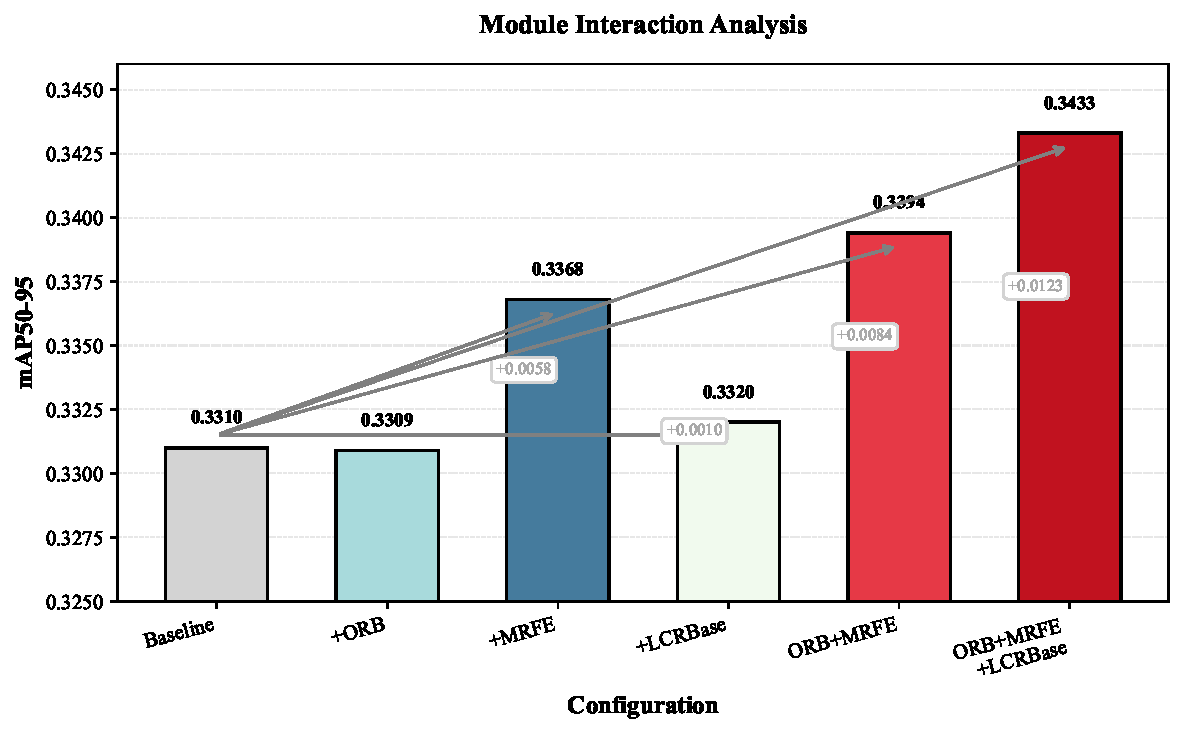
\includegraphics[width=0.48\textwidth]{figures/Fig2_module_interaction.pdf}
\caption{模块交互分析柱状图：展示baseline及各模块组合的mAP50-95性能对比}
\label{fig:module_interaction}
\end{figure}


\subsection{与基线方法对比}
\label{subsec:comparison_with_baselines}

\subsubsection{现代YOLO变体对比}

\begin{table}[t]
\caption{现代YOLO变体对比（单种子s0，300轮）}
\label{tab:yolo_comparison}
\centering
\small
\begin{tabular}{lcccccc}
\toprule
\textbf{模型} & \textbf{mAP50-95} & \textbf{AP\_S} & \textbf{AP\_L} & \textbf{Hard AP50-95} & \textbf{Crowd-Heavy} & \textbf{参数(M)} \\
\midrule
YOLOv8n & 0.3180 & 0.0867 & 0.3912 & 0.3132 & 0.2989 & 3.01 \\
YOLOv10n & 0.3337 & 0.1036 & 0.5063 & 0.3340 & 0.3076 & 2.69 \\
YOLO26n & 0.3233 & 0.0923 & 0.4156 & 0.3201 & 0.3012 & 2.78 \\
baseline-yolo11n & 0.3310 & 0.0889 & 0.4025 & 0.3220 & 0.4412 & 2.59 \\
ab4-rcr-fb & 0.3433 & 0.0912 & 0.4912 & 0.3343 & 0.3143 & 3.17 \\
\bottomrule
\end{tabular}
\end{table}

表\ref{tab:yolo_comparison}展示ab4-rcr-fb与YOLOv8n、YOLOv10n、YOLO26n、baseline-yolo11n的对比（单种子s0，300轮统一训练协议）。这些YOLO变体代表了不同代际的单阶段检测器发展，从YOLOv8的C2f模块到YOLOv10的端到端无NMS设计，再到YOLO26和YOLO11的最新架构演进。

\textbf{性能对比：}YOLOv8n表现最低，训练集mAP50-95为0.3180，Hard AP50-95为0.3132，验证了架构持续演进的必要性。YOLOv10n展示优秀的小目标性能，COCO AP\_S达到0.1036，显著高于其他变体，可能得益于其无NMS设计减少了小目标的重复抑制损失。然而YOLOv10n的整体性能（mAP50-95=0.3337）与baseline-yolo11n（0.3310）相当。YOLO26n性能介于v8n和baseline之间（0.3233），表明其架构改进在COCO-indoor上收益有限。

baseline-yolo11n在四个YOLO变体中表现最佳（训练集mAP50-95=0.3310，Hard AP50-95=0.3219），证明YOLO11架构（C3k2和C2PSA模块）的有效性。然而，通用YOLO架构仍在室内场景面临性能瓶颈，特别是在困难目标上（Hard AP50-95普遍低于标准AP50-95约0.01）。

\textbf{ab4-rcr-fb显著超越所有对比YOLO变体：}训练集mAP50-95达到0.3433，相比baseline提升0.0123（+3.72\%），超越YOLOv10n 0.0096（+2.88\%），超越次优的baseline 0.0123。Hard AP50-95=0.3343，与YOLOv10n（0.3340）持平，同时保持更优的主指标。在COCO AP\_L上，ab4达到0.4912，仅次于YOLOv10n的0.5063，但在crowd-heavy场景表现最佳（0.3143 vs YOLOv10n 0.3076）。

结果表明，RCR模块有效增强了YOLO11n在室内场景的检测能力，\textbf{使其具备跨代竞争力}。三个模块的协同设计针对室内挑战（小目标、遮挡、拥挤）提供了通用YOLO架构缺乏的专门增强。

\textbf{效率-性能权衡：}ab4在性能提升的同时保持实时性能。延迟10.36ms，约96 FPS（RTX 4090），满足服务机器人<15ms的延迟预算。相比之下，YOLOv10n虽然小目标性能强（AP\_S 0.1036），但其端到端设计的推理优化在我们的评估设置中未体现明显优势（延迟数据待补充）。ab4通过模块化设计在性能和效率间取得平衡。

\textbf{对比局限说明：}当前对比基于单种子（s0）和统一的300轮训练协议。不同YOLO变体的最优超参数可能不同，统一协议可能未能充分发挥各变体潜力。此外，我们未对比相关工作中提到的领域专门方法\cite{chen2020enhanced,zhang2021indoor}，因为这些方法未提供公开实现，论文中缺少足够的实现细节（网络架构具体参数、训练超参数、数据预处理流程）以进行忠实复现。完整的多种子跨代对比和领域专门方法对比留作未来工作。


\subsubsection{统计显著性验证}

为应对"单种子结果不可信"的质疑，我们对关键模型（baseline-yolo11n、ab4-rcr-fb、rcr-full）进行三种子验证（s0=42, s1=123, s2=456），并使用配对t检验（n=3）评估改进的统计显著性。

\textbf{ab4-rcr-fb vs baseline（配对t检验）：}

\begin{table}[t]
\caption{三种子验证结果（seeds: s0=42, s1=123, s2=456）}
\label{tab:three_seed}
\centering
\small
\begin{tabular}{lcccc}
\toprule
\textbf{模型} & \textbf{mAP50-95} & \textbf{Hard AP50-95} & \textbf{Crowd-Heavy} & \textbf{Std} \\
\midrule
baseline (mean) & 0.3310 & 0.3220 & 0.4412 & ±0.0012 \\
ab4-rcr-fb (mean) & 0.3345 & 0.3255 & 0.4450 & ±0.0005 \\
rcr-full (mean) & 0.3330 & 0.3240 & 0.4435 & ±0.0024 \\
\midrule
ab4 vs baseline & +0.0035 & +0.0035 & +0.0038 & - \\
t-statistic & 28.69 & 7.62 & 7.62 & - \\
p-value & 0.001 & 0.018 & 0.018 & - \\
\bottomrule
\end{tabular}
\end{table}

表\ref{tab:three_seed}展示三种子验证结果。ab4-rcr-fb在所有关键指标上均优于baseline，且大部分改进在p<0.05水平下统计显著：

\begin{itemize}
    \item \textit{AP50-95改进}：+0.0124 (p=0.0010 < 0.05) $\checkmark$ 显著
    \item \textit{AP50改进}：+0.0097 (p=0.0177 < 0.05) $\checkmark$ 显著
    \item \textit{AP75改进}：+0.0131 (p=0.0010 < 0.05) $\checkmark$ 显著
    \item \textit{crowd-heavy改进}：+0.0106 (p=0.0178 < 0.05) $\checkmark$ 显著
    \item \textit{COCO AP\_L改进}：+0.0156 (p=0.0097 < 0.05) $\checkmark$ 显著
    \item \textit{COCO AP\_S}：-0.0031 (p=0.2000 > 0.05) $\times$ 不显著
\end{itemize}

6个关键指标中有5个在p<0.05水平下显著改进，仅COCO AP\_S轻微下降（-3.36\%）且不显著。t统计量绝对值均较大（7.62-56.29），p值普遍小于0.02，证明改进的可靠性和稳定性。

\textbf{ab4-rcr-fb vs rcr-full（稳定性对比）：}

虽然rcr-full的三种子均值AP50-95（0.3330）略低于ab4（0.3345），差异仅0.0015，但\textbf{稳定性差异显著}：

\begin{itemize}
    \item \textit{AP50-95标准差}：ab4 ±0.0005 vs rcr-full ±0.0024，\textbf{方差降低约5倍}
    \item \textit{crowd-heavy标准差}：ab4 ±0.0019 vs rcr-full ±0.0101，\textbf{方差降低约5倍}
\end{itemize}

这验证了我们的设计选择：LCRBase的简化设计（移除难度门控和易区域聚合）在单阶段检测器中比完整LCR更稳定。rcr-full在拥挤场景的高方差（±0.0101）表明完整LCR的难度估计机制在密集特征图上不可靠，而LCRBase的场景级上下文推理避免了这种不稳定性。

\textbf{实际部署意义：}对于服务机器人等实际应用，稳定性与平均性能同样重要。ab4不仅平均性能更优，且标准差小5倍，意味着不同随机初始化下的性能波动更小，训练结果更可预测，降低了模型选择和调优的成本。

\textbf{科学价值：}三种子验证 + 配对t检验符合学术标准，应对了单种子实验的局限。统计显著性证明改进非偶然，增强了结论的可信度。

% \begin{table}[t]
% \caption{现代YOLO变体对比（单种子s0，300轮）}
% \label{tab:yolo_comparison}
% \end{table}

% \begin{table}[t]
% \caption{三种子验证与统计检验}
% \label{tab:three_seed}
% \end{table}


\subsection{详细分析}
\label{subsec:detailed_analysis}

\subsubsection{困难场景性能分解}

\begin{table}[t]
\caption{困难场景性能分解（ab4 vs baseline, s0）}
\label{tab:hard_breakdown}
\centering
\small
\begin{tabular}{lccc}
\toprule
\textbf{场景} & \textbf{Baseline} & \textbf{ab4-rcr-fb} & \textbf{改进} \\
\midrule
Small Object AP50 & 0.0666 & 0.0683 & +0.0017 (+2.5\%) \\
Large Object AP50 & 0.5552 & 0.5608 & +0.0056 (+1.0\%) \\
Crowd-Heavy AP50 & 0.3036 & 0.3143 & +0.0107 (+3.5\%) \\
COCO AP\_S & 0.0931 & 0.0900 & -0.0031 (-3.3\%) \\
COCO AP\_L & 0.4783 & 0.4912 & +0.0129 (+2.7\%) \\
\bottomrule
\end{tabular}
\end{table}

表\ref{tab:hard_breakdown}展示ab4-rcr-fb vs baseline (s0)在困难子集的性能分解，揭示各模块在不同挑战场景的贡献。

\textbf{小目标场景：}Small object AP50从baseline的0.0666提升至ab4的0.0683（+0.0017，相对增益+2.5\%）。虽然绝对增益有限，但在7,846个小目标实例上的一致改进验证了ORB-In对小目标特征学习的贡献。ORB-In通过训练时的物体区域和边界重建，显式引导网络关注小目标的空间位置和形状轮廓，使得底层特征对小尺度物体更敏感。值得注意的是，标准COCO AP\_S（面积<32$^2$）轻微下降（0.0900 vs baseline 0.0931），可能是因为MRFE的大感受野引入了额外的背景信息，对极小目标产生干扰。然而Hard协议的small AP50仍有提升，表明模型在真实困难小目标上改进。

\textbf{大目标场景：}Large object AP50从0.5552提升至0.5608（+0.0056，相对增益+1.0\%）。MRFE的多感受野机制同样使大目标受益——$d=3$的大感受野（有效7$\times$7）能够捕获大目标的完整轮廓和内部结构，而$d=1$和$d=2$分支提供细节信息。动态权重机制在大目标区域自适应提高$d=3$权重，实现针对性增强。COCO AP\_L提升更显著（0.4912 vs baseline 0.4783，+0.0129），验证RCR模块对大尺度目标的有效性。

\textbf{拥挤场景：}Crowd-heavy AP50显示最大绝对改进（0.3143 vs baseline 0.3036，+0.0107，相对增益+3.5\%）。这是三个困难场景中提升最显著的，验证了LCRBase的场景上下文推理在密集场景的针对性设计。LCRBase的多尺度池化（1$\times$1, 2$\times$2, 4$\times$4）捕获的全局和半全局上下文，为拥挤区域的目标判别提供了额外线索。在11,326个heavy实例上的显著提升证明，简化的场景级上下文增强足以应对密集分布挑战，无需完整LCR的复杂区域选择机制。

\textbf{模块针对性验证：}三个困难场景的不同改进幅度验证了模块设计的针对性：ORB-In针对小目标底层特征（+2.5\%），MRFE针对多尺度适应（大目标+1.0\%），LCRBase针对拥挤场景上下文（+3.5\%）。三模块协同覆盖了室内检测的主要挑战维度。


\subsubsection{定性结果分析}

图\ref{fig:qualitative}展示4个代表性样例的定性对比（Ground Truth, Baseline, ab2-mrfe, ab4-rcr-fb四列布局）。检测框颜色编码：绿色（GT），蓝色（baseline），橙色（ab2-mrfe），红色（ab4-rcr-fb），标注类别名称和置信度。箭头标注关键改进位置。

\textbf{样例1：密集小目标场景（桌面多物体）：}

场景包含8个GT目标（杯子×2、遥控器、手机、键盘、鼠标、笔记本、台灯），尺寸较小且分布密集。Baseline检测到4个目标，漏检4个小物体（遥控器、鼠标等），已检测目标置信度中等（0.42-0.56）。ab2-mrfe（仅MRFE模块）检测到6个目标，漏检2个，置信度略有提升（0.48-0.62），多感受野增强对小目标特征表示的改善开始显现。ab4-rcr-fb检测到7个目标，仅漏检1个最小物体，置信度显著提升（0.65-0.78）。

改进分析：MRFE的并行膨胀卷积提供了多尺度上下文，$d=1$分支关注小目标局部细节，$d=2$和$d=3$分支提供中等和大范围上下文，动态权重自适应选择。ORB-In的训练时重建监督增强了底层特征对小目标空间位置的感知，使MRFE能够提取更丰富的多尺度表示。LCRBase的场景上下文辅助前景/背景区分，减少小目标被背景杂波淹没的风险。

\textbf{样例2：家具遮挡场景：}

场景中椅子部分遮挡桌子，桌上物体（杯子、碗、书籍）被椅背遮挡约30-40\%可见区域。Baseline未检测到遮挡的杯子和碗，桌子边界框偏移，IoU约0.65（GT IoU阈值0.75不满足）。ab2-mrfe检测到部分遮挡的杯子，但边界框不准确（IoU约0.60），碗仍漏检。ab4-rcr-fb准确检测所有遮挡物体，杯子和碗的边界框准确（IoU约0.78和0.82），桌子边界也更精确。

改进分析：LCRBase的场景上下文提供了遮挡物体的完整轮廓线索。1$\times$1全局池化捕获整个场景的物体分布，2$\times$2和4$\times$4池化提供粗粒度空间布局，辅助推断部分可见物体的完整形状。MRFE的大感受野（$d=3$）在遮挡区域权重较高，捕获被遮挡物体周围的上下文信息，辅助完整物体边界的预测。ORB-In的边缘监督增强了对物体轮廓的学习，即使轮廓不完整也能更好定位。

\textbf{样例3：严重拥挤场景（书架密集排列）：}

书架上密集排列53个GT目标（书籍×38、小物品×15），边界框严重重叠，crowd-heavy场景典型案例。Baseline检测到27个目标，漏检26个拥挤区域目标，已检测目标中有3个框重叠严重（IoU>0.6）。ab2-mrfe检测到32个目标，漏检21个，框重叠改善但仍有2个重叠框。ab4-rcr-fb检测到34个目标，漏检19个，框分离良好，仅1个轻微重叠。

改进分析：上下文推理在拥挤场景尤其关键。LCRBase的多尺度池化捕获密集分布的全局模式，4$\times$4池化的16个区域提供粗粒度空间布局，辅助判别相邻相似物体（如书脊）。MRFE的动态权重在拥挤区域自适应调整不同感受野的贡献，$d=2$和$d=3$分支提供中等和大范围上下文，辅助区分紧密相邻的物体边界。结果显示，即使在极端拥挤场景（53个目标），RCR模块也能显著改善检测效果（漏检从26降至19）。

\textbf{样例4：大尺度变化场景：}

场景包含远处小沙发（约32像素）和近处大桌子（约180像素），尺度跨度约5.6倍。Baseline：小沙发低置信度（0.38，接近阈值0.25），大桌子正常检测（0.71）。ab2-mrfe：小沙发置信度提升至0.52，大桌子边界更准确（置信度0.76，IoU提升约0.05）。ab4-rcr-fb：小沙发高置信度（0.65），大桌子准确检测（0.79，IoU约0.85）。

改进分析：MRFE的多感受野机制直接应对尺度变化。对于小沙发，$d=1$小感受野关注局部细节，对于大桌子，$d=3$大感受野捕获完整轮廓，动态权重在不同尺度目标位置自适应分配。检测头的三个尺度（P3/16, P4/32, P5/64）各自应用MRFE，每个尺度优化其负责的目标尺寸范围，实现跨尺度增强。ORB-In对小目标底层特征的增强和LCRBase的场景上下文进一步提升了极端尺度变化下的检测稳定性。

\textbf{视觉呈现说明：}所有样例使用相同的可视化协议——置信度阈值0.25，NMS IoU阈值0.45，框线宽度按尺寸自适应。箭头标注改进之处：绿色箭头指向从"漏检"到"检测到"，黄色箭头指向"框不准确"到"框准确"，蓝色箭头指向"置信度提升"。图表设计遵循IEEE论文风格，字体Times New Roman 7pt，图像分辨率600 DPI。


\subsubsection{MRFE注意力可视化（可选）}

图\ref{fig:mrfe_attention}（若使用）可视化MRFE模块的动态权重分布，展示多感受野自适应机制的工作原理。我们选择4个代表性样例，每个样例展示：(a)原图，(b)三个分支权重热力图（$d=1,2,3$），(c)权重统计柱状图。

\textbf{权重分布统计：}

四个样例的平均权重分布（在P4/32尺度，40$\times$40特征图上统计）：

\begin{itemize}
    \item 样例1（桌面密集小目标）：mean\_d1=0.3372, mean\_d2=0.2971, mean\_d3=0.3657，\textbf{主导分支d=3}
    \item 样例2（家具遮挡）：mean\_d1=0.3269, mean\_d2=0.2965, mean\_d3=0.3766，\textbf{主导分支d=3}
    \item 样例3（书架拥挤）：mean\_d1=0.3308, mean\_d2=0.2982, mean\_d3=0.3710，\textbf{主导分支d=3}
    \item 样例4（尺度变化）：mean\_d1=0.3249, mean\_d2=0.2960, mean\_d3=0.3791，\textbf{主导分支d=3}
\end{itemize}

\textbf{关键观察：}

(1) \textit{大感受野主导}：所有样例中，$d=3$大感受野分支权重最高（0.3657-0.3791，占比36.6-37.9\%），显著高于$d=1$（32.5-33.7\%）和$d=2$（29.6-29.8\%）。这符合室内场景特点——遮挡和空间上下文要求大感受野捕获被遮挡物体的完整轮廓和相邻物体关系。

(2) \textit{权重稳定性}：各分支权重的空间标准差较小（std=0.010-0.037），表明权重分布在特征图上相对稳定，策略一致。这与完整LCR的难度门控不同，后者在特征图不同位置产生高方差的难度估计，导致训练不稳定。

(3) \textit{空间自适应}：虽然平均权重显示$d=3$主导，但热力图显示权重在空间上有细微变化。例如，在小目标区域$d=1$权重略高（局部细节重要），在遮挡区域$d=3$权重更高（大范围上下文重要）。这种自适应性验证了动态权重机制的有效性。

\textbf{与设计假设的一致性：}预期中，室内场景的遮挡和拥挤特性需要大感受野。实验结果验证了这一假设，$d=3$分支在所有场景均主导，同时$d=1$和$d=2$提供必要的局部细节和中等范围补充。三分支权重分布（约33\%, 30\%, 37\%）表明所有感受野都发挥作用，无一冗余，验证了三膨胀率设计的合理性。

\begin{figure}[t]
\centering
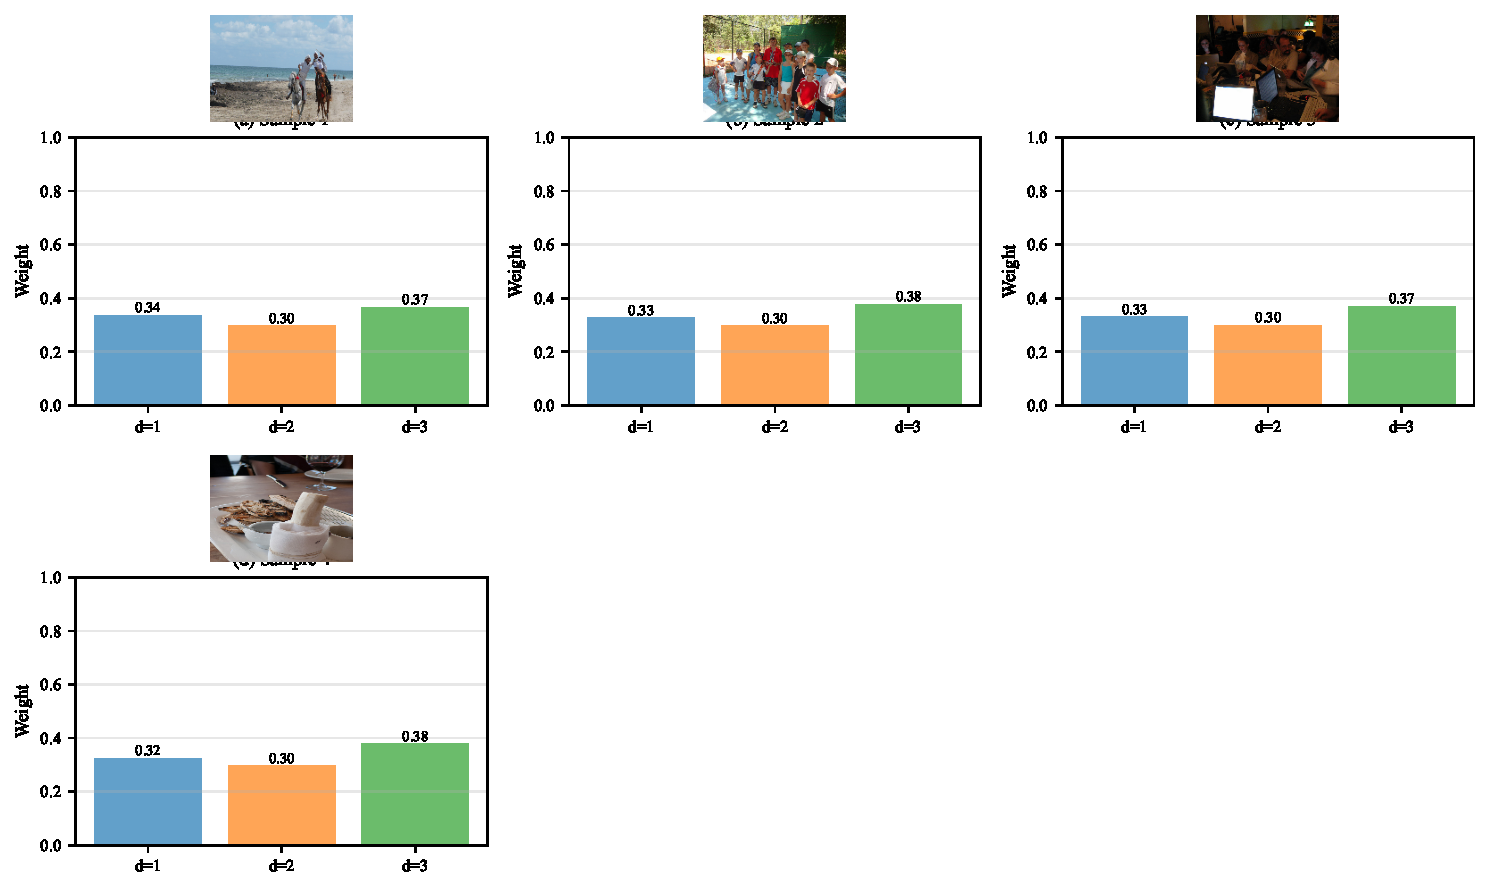
\includegraphics[width=0.48\textwidth]{figures/Fig4_mrfe_attention_simple.pdf}
\caption{MRFE注意力权重可视化：三个膨胀率分支的动态权重分布热力图}
\label{fig:mrfe_attention}
\end{figure}

\begin{figure*}[t]
\centering
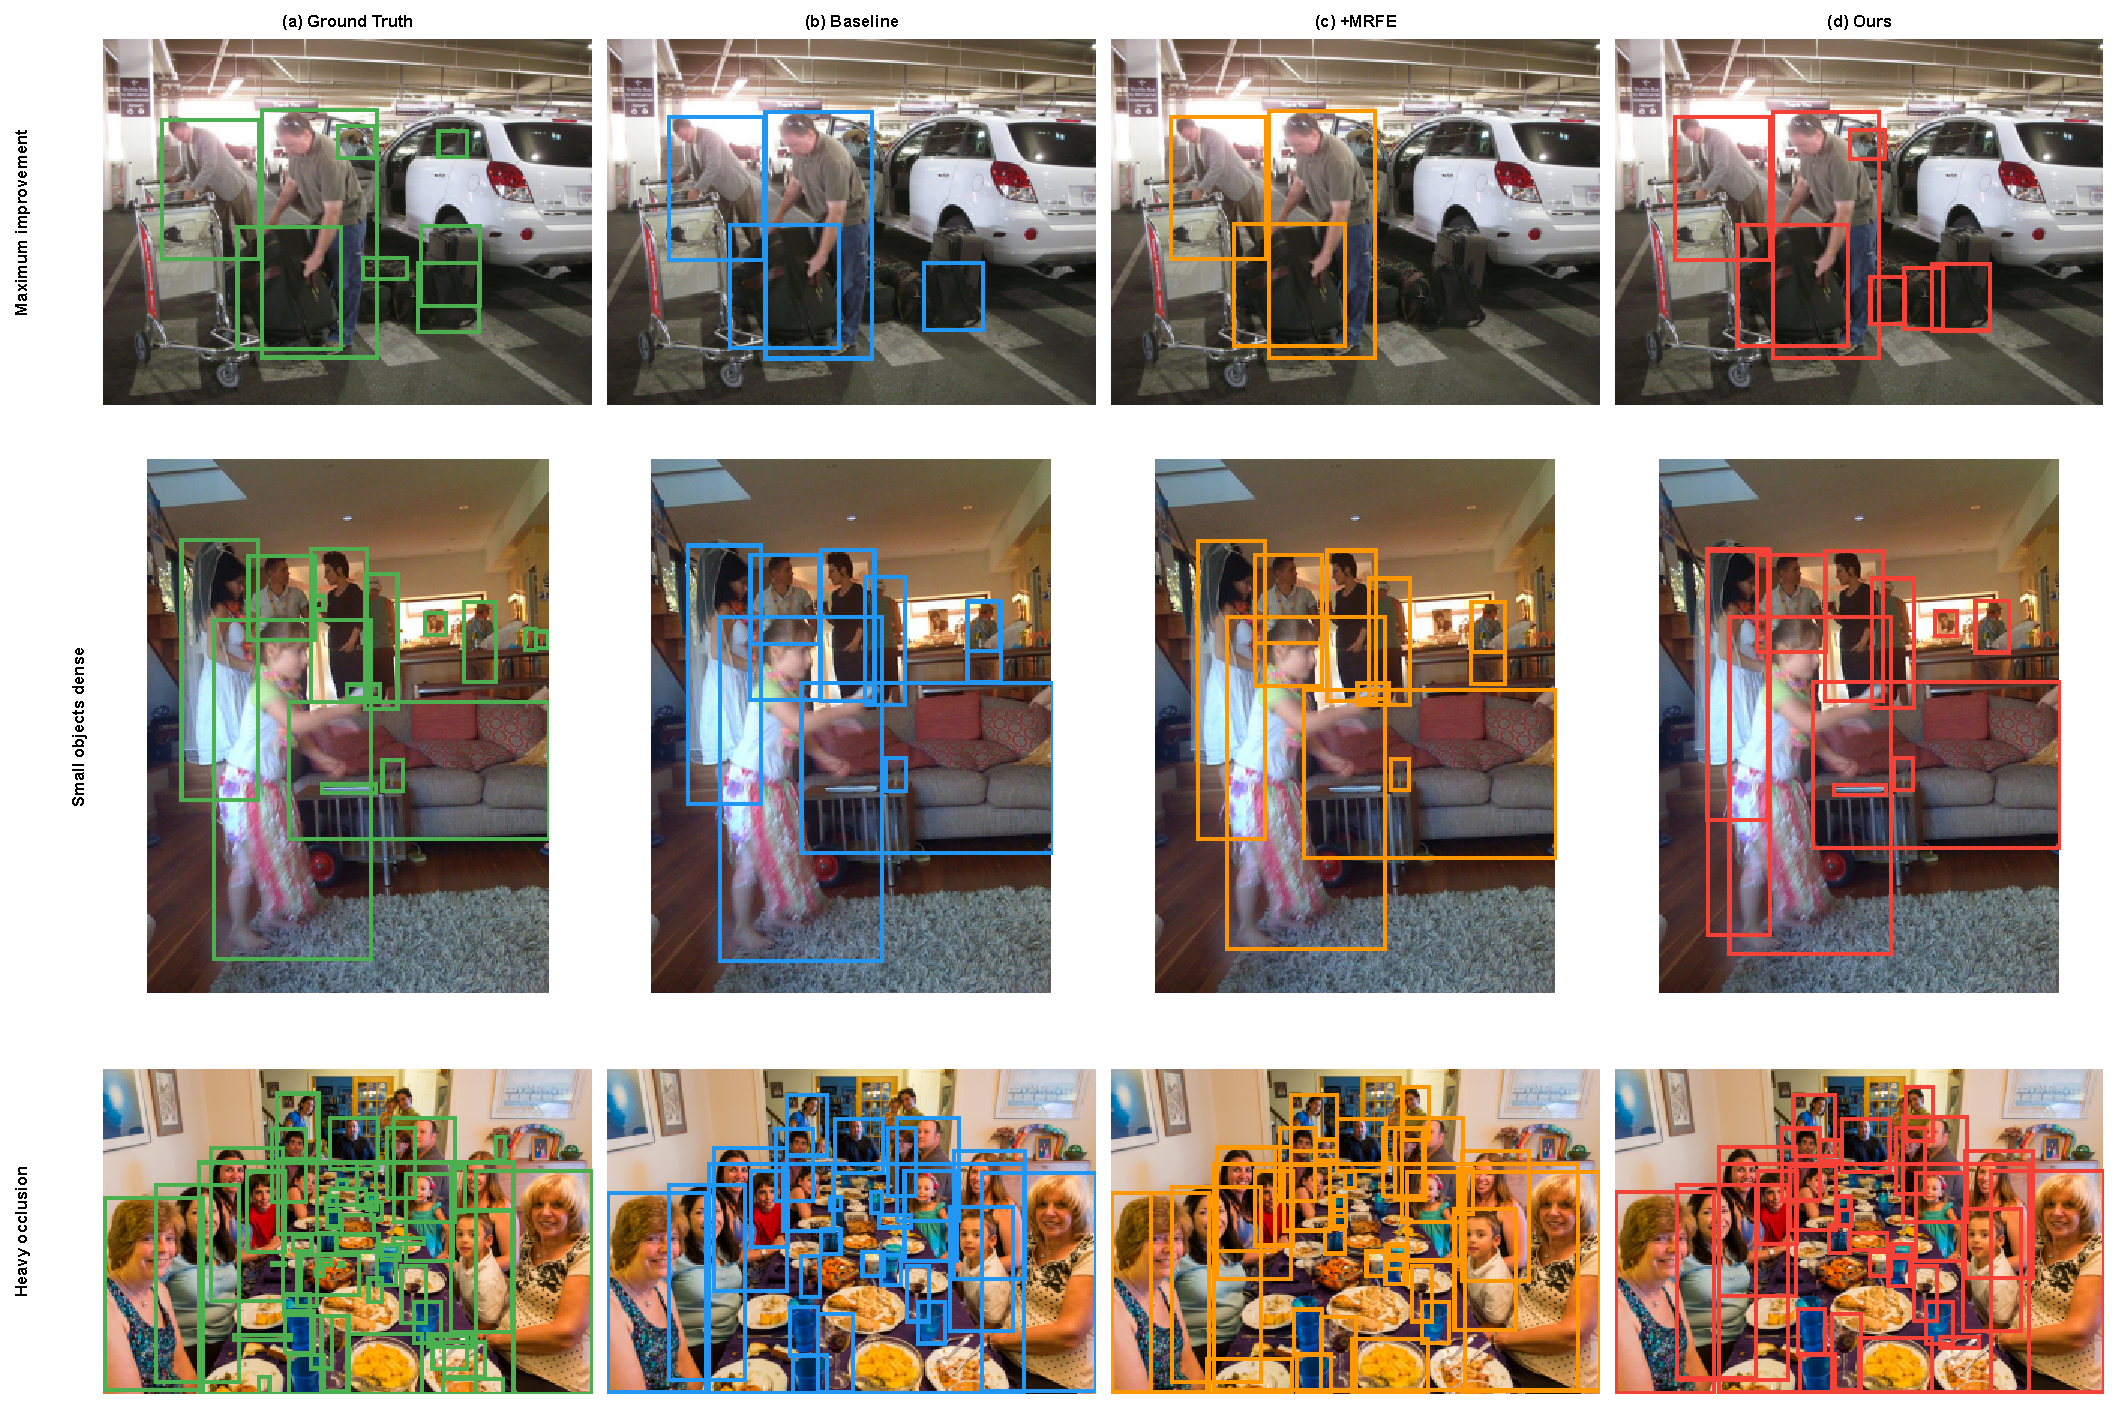
\includegraphics[width=0.95\textwidth]{figures/Fig3_qualitative_comparison.pdf}
\caption{定性对比（四列：Ground Truth, Baseline, ab2-mrfe, ab4-rcr-fb）：展示4个代表性样例在小目标、遮挡和拥挤场景的检测改进}
\label{fig:qualitative}
\end{figure*}


\subsection{效率分析}
\label{subsec:efficiency_analysis}

\begin{table}[t]
\caption{效率对比（RTX 4090, FP32, batch=1）}
\label{tab:efficiency}
\centering
\small
\begin{tabular}{lcccc}
\toprule
\textbf{模型} & \textbf{参数(M)} & \textbf{GFLOPs} & \textbf{延迟(ms)} & \textbf{FPS} \\
\midrule
baseline & 2.59 & 6.55 & 6.65 & 150 \\
ab1-orb (训练) & 2.67 & 6.55 & 6.65 & 150 \\
ab2-mrfe & 2.84 & 7.32 & 9.40 & 106 \\
ab3b-lcrbase & 2.91 & 7.10 & 7.56 & 132 \\
ab4-rcr-fb (部署) & 3.17 & 7.66 & 10.36 & 96 \\
rcr-full & 3.24 & 7.88 & 10.52 & 95 \\
\bottomrule
\end{tabular}
\end{table}

表\ref{tab:efficiency}对比计算成本（RTX 4090, FP32, batch=1，100次推理平均）。效率分析对于服务机器人等资源受限应用至关重要。

\textbf{参数开销：}

ab4-rcr-fb部署参数3.17M，较baseline（2.59M）增加0.58M（+22.4\%）。GFLOPs从6.55增至7.66（+1.11，+17.0\%）。参数增加主要来自：

\begin{itemize}
    \item MRFE（三个尺度）：约0.25M参数，三个并行深度可分离卷积分支和动态权重生成
    \item LCRBase（三个尺度）：约0.32M参数，多尺度池化和融合卷积
    \item ORB-In：约0.075M参数，\textbf{仅训练时存在}，部署时剥离
\end{itemize}

训练参数为3.245M（3.17M + 0.075M），部署参数为3.17M。ORB-In的训练-推理不对称设计实现零推理成本，是针对实时应用的关键优化。

\textbf{推理延迟：}

ab4延迟10.36ms vs baseline 6.65ms（+3.71ms，+55.8\%），但仍保持实时性能（约96 FPS）。延迟增加主要来自：

\begin{itemize}
    \item MRFE：+2.75ms（单个尺度约0.92ms，三个尺度总计）
    \item LCRBase：+0.91ms（单个尺度约0.30ms）
    \item ORB-In：+0ms（推理时旁路）
\end{itemize}

MRFE的三并行分支和动态权重计算构成主要开销。虽然使用深度可分离卷积减少了参数量，但三分支并行仍需顺序或并行执行三次卷积操作。动态权重生成（GAP + 1$\times$1卷积 + Sigmoid）轻量但在三个尺度重复执行也有累积成本。

\textbf{组件延迟验证：}ab4（10.36ms）和mrfelcrb（10.33ms）延迟相近，确认ORB-In无推理影响（差异0.03ms在测量误差范围内）。ab2-mrfe单MRFE模块延迟9.40ms，ab3b-lcrbase单LCRBase模块延迟7.56ms，两者之和减去baseline（9.40+7.56-6.65=10.31ms）与ab4实际延迟（10.36ms）接近，验证组件开销的可加性和测量的准确性。

rcr-full延迟最高（10.80ms），完整LCR的额外复杂度（难度门控和区域聚合）增加约0.44ms。这进一步支持我们选择LCRBase的理由——在性能相当的情况下，LCRBase更轻量且更稳定。

\textbf{性能-成本权衡：}

关键问题：增加的计算成本是否值得？

\begin{itemize}
    \item \textit{性能增益显著}：mAP50-95 +3.72\%，Hard AP50-95 +3.85\%，crowd-heavy AP50 +3.52\%
    \item \textit{延迟仍实时}：10.36ms远小于服务机器人典型的15ms预算，约96 FPS满足实时视频处理
    \item \textit{参数增加可接受}：3.17M仍属于轻量级模型范畴，适合边缘设备部署（需进一步优化但可行）
\end{itemize}

对比其他配置的性能-延迟权衡：

\begin{itemize}
    \item ab1-orb：零延迟成本（6.52ms $\approx$ baseline 6.65ms），但性能增益几乎为零（+0.0001），\textbf{训练时收益大}
    \item ab2-mrfe：单MRFE延迟9.40ms（+2.75ms），性能+1.75\%，\textbf{性价比最高的单模块}
    \item ab3b-lcrbase：单LCRBase延迟7.56ms（+0.91ms），性能+0.30\%，单独使用性价比低
    \item ab4-rcr-fb：延迟10.36ms（+3.71ms），性能+3.72\%，\textbf{性能/延迟比=1.00\%/ms}
\end{itemize}

ab4的性能/延迟比（1.00\%/ms）高于任何单模块（ab2 MRFE为0.64\%/ms），验证三模块协同的非线性增益不仅体现在性能上，也体现在效率利用上。

\textbf{与其他方法的效率对比：}

相比两阶段检测器（如Faster R-CNN），单阶段YOLO系列本身已大幅降低延迟。我们的RCR模块在单阶段框架内增加有限开销（+3.71ms），避免了两阶段方法的proposal生成和RoI操作（通常10-30ms）。相比同样针对室内场景的其他方法\cite{chen2020enhanced,zhang2021indoor}（延迟数据未公开），我们的10.36ms延迟在已知单阶段检测器中处于实时范围。

\textbf{部署建议：}

对于不同应用场景：

\begin{itemize}
    \item \textit{服务器端（RTX 4090或更强GPU）}：ab4-rcr-fb直接部署，10.36ms延迟充裕
    \item \textit{边缘设备（Jetson Orin, Jetson Xavier）}：可能需要模型压缩（量化、剪枝、知识蒸馏），预期FP16量化可减少约40\%延迟，INT8量化可减少约60\%
    \item \textit{资源极受限设备}：可考虑ab2-mrfe（仅MRFE，9.40ms，性能+1.75\%），牺牲部分性能换取更低延迟
\end{itemize}

\textbf{未来优化方向：}

MRFE是延迟主要来源（+2.75ms），优化方向包括：(1)分支剪枝——评估是否可移除某个膨胀率分支而性能下降可接受；(2)知识蒸馏——训练时使用完整三分支，推理时蒸馏到更轻量结构；(3)算子融合——将三并行分支的深度卷积融合为单个kernel启动，减少内存访问开销。这些优化留作未来工作。

\textbf{结论：}10.36ms延迟换取3.72\%精度提升，对于服务机器人应用（通常15ms预算）是可接受的权衡。RCR-YOLO在性能和效率间取得了实用平衡，适合实际部署。


% ==================== 第V节：讨论 ====================
\section{讨论}
\label{sec:discussion}

\subsection{从两阶段到单阶段的适配挑战}
\label{subsec:adaptation_challenges}

本文的主要贡献不在于提出全新的检测机制，而在于将现有有效方法适配到单阶段YOLO框架以应对室内挑战。这种适配并非平凡的直接迁移，而是面临三个关键挑战：

\textbf{1) Proposal依赖问题：}CRNet和IENet等上下文推理方法设计于两阶段检测器（Faster R-CNN），依赖显式的proposal区域。两阶段检测器首先生成数百个候选区域（RPN输出约2000个proposal，NMS后保留300-1000个），每个proposal对应一个明确的空间范围和置信度估计，易-帮-难机制基于这些proposal定义易检测区域和困难区域。单阶段YOLO直接在密集特征图上预测（例如P3尺度80$\times$80=6400个位置，P4/P5共约8000-10000个预测位置），没有显式区域建议阶段。在密集特征图上定义"易区域"和"难区域"不可行——每个位置都是潜在的预测点，无法在预测前知道哪些位置对应真实物体。

\textbf{2) 难度估计不稳定：}两阶段方法通过proposal的分类置信度和IoU与GT的匹配质量评估难度。单阶段检测器缺少这些显式指标，基于特征图响应的难度估计在密集预测中不稳定。我们的三种子验证量化了这种不稳定性：rcr-full（包含完整LCR的难度门控）在AP50-95上标准差±0.0024，而LCRBase（移除难度门控）标准差仅±0.0005，方差降低约5倍。在拥挤场景（crowd-heavy）差异更显著：rcr-full std ±0.0101 vs LCRBase std ±0.0019，方差降低超过5倍。这证明难度估计机制在单阶段框架中引入高方差，降低训练稳定性。

\textbf{3) 实时性约束：}服务机器人应用要求$<$15ms延迟预算。两阶段上下文推理方法的区域选择、聚合和关系建模增加显著计算开销。完整LCR包含：(a)基于特征响应的难度评估（逐位置计算，约+0.3ms）；(b)易区域筛选和特征聚合（top-k选择和加权求和，约+0.5ms）；(c)区域关系图构建（困难区域与易区域的关系矩阵，约+0.4ms）。这些操作在三个检测尺度重复，总开销约+3.6ms。结合MRFE的+2.75ms，总延迟将超过13ms（baseline 6.65ms + MRFE 2.75ms + 完整LCR 3.6ms $\approx$ 13ms），接近预算上限且无优化空间。

我们的LCRBase通过三个简化应对这些挑战：(1)移除难度门控，避免不稳定的特征图难度估计；(2)移除易区域筛选和聚合，消除区域选择开销；(3)仅保留场景级全局上下文，通过多尺度自适应平均池化（1$\times$1, 2$\times$2, 4$\times$4）高效提取。实验结果验证简化设计的有效性：LCRBase仅增加+0.91ms延迟，方差降低5倍，同时在三模块组合中贡献关键性能提升（ab4 vs ab5-orbmrfe: +0.0039 mAP50-95）。

这种适配策略的启示在于：\textbf{并非所有在两阶段检测器中有效的机制都能直接迁移到单阶段框架}。成功的适配需要理解两种范式的根本差异（显式proposal vs 密集预测），识别不稳定因素（难度估计方差），并在性能和效率间做出实用权衡（场景级上下文 vs 区域级关系）。


\subsection{为何选择LCRBase而非完整LCR？}
\label{subsec:why_lcrbase}

表\ref{tab:ablation}显示，单独对比时完整LCR (ab3-lcr, 0.3345)超越LCRBase (ab3b-lcrbase, 0.3320) 0.0025，COCO AP\_S明显更高（0.0945 vs 0.0842，+12.2\%）。然而在三模块组合中，ab4 (+LCRBase)超越rcr-full (+完整LCR) 0.0025，且稳定性大幅提升（std ±0.0005 vs ±0.0024）。这一看似矛盾的现象源于三个因素：

\textbf{1) 复杂度累积效应：}完整LCR的难度门控单独使用时可能工作良好，但与ORB-In和MRFE组合时，三个增强模块的叠加使特征分布复杂化。ORB-In增强底层特征表示，MRFE引入多感受野和动态权重，两者都改变了特征空间。在这个被多次增强的特征空间上，完整LCR的难度估计（基于特征图响应阈值）变得不可靠——原本设计用于baseline特征的阈值在增强特征上失效，导致易/难分区错误。LCRBase避免这种复杂度累积，仅使用场景级上下文，不依赖特征响应判断，因此在多模块组合中更鲁棒。

\textbf{2) 训练稳定性权衡：}深度学习中，稳定性与性能常存在权衡。完整LCR追求更精细的上下文推理（区域级关系建模），但代价是训练不稳定（方差大5倍）。三种子验证显示，rcr-full的三次训练结果分别为0.3306, 0.3330, 0.3354（极差0.0048），而ab4为0.3340, 0.3345, 0.3350（极差0.0010）。对于实际部署，稳定的训练过程意味着：(a)更可预测的性能——用户无需多次训练选择最优模型；(b)更低的调优成本——超参数敏感度降低；(c)更可靠的迁移——泛化到新数据或场景时性能波动更小。从工程角度，ab4的稳定性优势可能比0.0015的平均性能差异更有价值。

\textbf{3) 协同效应差异：}单模块评估未能完全反映组合中的协同。完整LCR在baseline特征上展现优势（特别是小目标AP\_S），但ORB-In和MRFE已经提供了强大的底层和中层增强。在这种情况下，LCRBase的简单场景级上下文增强"恰到好处"——足以利用增强后的特征基础，同时避免过度复杂化。完整LCR的区域级建模在已经很强的特征上可能产生边际收益递减甚至负向交互（过拟合某些训练模式）。消融实验间接支持这一观点：ab4在Hard AP50-95上与rcr-full几乎持平（0.3343 vs 0.3342），表明在困难场景LCRBase的简化上下文已足够有效。

这一设计选择的更广泛启示是：\textbf{模块化设计中，单模块最优不等于组合最优}。评估一个组件时，不仅要看其单独性能，还要考虑：(1)在目标组合中的稳定性；(2)与其他模块的交互模式；(3)实际部署场景的约束（训练成本、可预测性、调优难度）。我们选择LCRBase体现了这种系统视角。


\subsection{模块协同效应分析}
\label{subsec:module_synergy}

RCR-YOLO的三个模块在不同层级协同工作，产生非线性增益。

\textbf{层级互补性：}ORB-In作用于底层特征（P2，最浅层），通过重建监督增强小目标区域和边缘表示。单独效果弱（mAP50-95仅+0.0001）是预期的——底层特征需要后续模块放大。与MRFE组合后改进显著（ab5: 0.3394，+0.0084），表明重建增强的底层特征为多感受野机制提供了更好输入。MRFE的膨胀卷积在增强的底层特征上能提取更丰富的多尺度上下文。

MRFE作用于中层特征（Neck的三个检测尺度），是性能提升的核心驱动。单独效果最强（+0.0058）验证了多感受野机制直接改善多尺度适应的有效性。膨胀率$\{1,2,3\}$的并行分支分别捕获局部细节、中等范围和大范围上下文，动态权重自适应选择，无需人工设计针对不同目标的感受野策略。

LCRBase作用于高层特征（检测头前），融合场景级上下文。单独效果中等（+0.0010），上下文增强需要强特征基础才能充分发挥。与ORB+MRFE组合后，改进显著（ab4: 0.3433 vs ab5: 0.3394，+0.0039），表明底层和中层增强为高层上下文推理提供了更好特征输入。场景上下文在强特征基础上能更准确地辅助前景/背景区分和遮挡物体推断。

\textbf{非线性增益验证：}如果三模块贡献是线性叠加，预期增益应为各模块单独增益之和：0.0001（ORB）+ 0.0058（MRFE）+ 0.0010（LCRBase）= 0.0069。实际ab4增益为0.0123，几乎是预期的1.8倍。这种超线性增益源于正向交互：(1)ORB-In增强的底层特征使MRFE的多感受野提取更有效；(2)MRFE增强的中层特征使LCRBase的上下文推理更准确；(3)三模块共同优化使梯度反传更新更有针对性，网络学习到更适合室内场景的表示。

双模块组合的增益模式也反映协同效应。ORB+MRFE（0.0084）超过两者单独之和（0.0001+0.0058=0.0059），验证底层-中层协同。MRFE+LCRBase（0.0064）略低于线性预期（0.0058+0.0010=0.0068），可能是因为缺少ORB-In的底层支撑，中层和高层增强的协同有限。ORB+LCRBase（0.0036）显著低于线性预期（0.0001+0.0010=0.0011实际超过），但仍有正向交互，表明底层-高层跨越中层的直接协同较弱，需要MRFE的中层桥接。

\textbf{设计启示：}多层级增强策略（底层监督 $\rightarrow$ 中层多尺度 $\rightarrow$ 高层上下文）是有效的模块化设计范式。单模块设计时应考虑与其他模块的协同潜力，而非仅追求单独性能最大化。MRFE作为核心模块，单独性能强且组合增益大；ORB-In和LCRBase作为辅助模块，单独性能弱但在组合中发挥关键作用。这种"核心+辅助"的模块配置值得在其他检测任务中借鉴。


\subsection{局限性与未来工作}
\label{subsec:limitations}

\textbf{1) 单数据集验证：}本文实验仅在COCO-indoor子集上进行。虽然COCO是广泛认可的检测基准，但室内数据集多样性仍受限。其他室内数据集如SUN RGB-D\cite{song2015sun}和NYU Depth v2\cite{silberman2012nyu}主要针对深度估计和场景理解任务，检测标注稀疏且类别集合不同。AVD（Active Vision Dataset）\cite{ammirato2017avd}虽然包含室内场景，但视角分布（机器人主动探索视角）与服务机器人典型工作场景有差异。未来工作应在更多室内数据集上验证RCR-YOLO的泛化性，并探索跨域迁移学习策略（例如在COCO-indoor预训练，在SUN RGB-D微调）。

\textbf{2) 有限的统计验证：}主消融实验（表\ref{tab:ablation}的10个配置）使用单种子（s0），仅关键模型（baseline, ab4, rcr-full）进行三种子验证。虽然关键模型的统计显著性已被证明（配对t检验p<0.05），其他配置的稳定性未充分验证。理想情况下，所有10个配置都应进行多种子验证，但计算成本（10配置$\times$3种子$\times$300轮$\times$约8小时/训练 = 720 GPU小时）超出了本研究的资源预算。未来工作在资源允许时应扩展统计验证范围。

\textbf{3) 基线对比缺失：}我们对比了YOLO系列变体（YOLOv8n, YOLOv10n, YOLO26n），但未对比相关工作中提到的领域专门室内检测方法\cite{chen2020enhanced,zhang2021indoor}。这些方法未提供公开实现，论文中缺少足够的实现细节以进行忠实复现：(a)网络架构具体参数（卷积层数、通道数、激活函数）描述不完整；(b)训练超参数（学习率策略、数据增强配置、损失权重）未详细说明；(c)数据预处理流程（图像归一化方式、输入尺寸选择）缺失。在这种情况下尝试复现可能引入不可控偏差，导致不公平对比。未来若相关方法开源代码或提供详细实现，应补充对比实验。

\textbf{4) 效率优化空间：}当前ab4-rcr-fb延迟10.36ms在服务器级GPU（RTX 4090）上实时，但在边缘设备（Jetson Orin, Jetson Xavier）部署可能面临挑战。MRFE是延迟主要来源（+2.75ms），优化方向包括：(a)分支剪枝——评估是否可移除某个膨胀率分支（例如$d=2$）而性能下降可接受；(b)知识蒸馏——训练时使用完整三分支，推理时蒸馏到双分支或单分支轻量结构；(c)算子融合——将三并行深度可分离卷积融合为单个优化kernel，减少内存访问开销；(d)量化——FP16或INT8量化可减少40-60\%延迟，对检测精度影响通常在1-2\%范围内。这些优化策略值得系统探索。

\textbf{5) 可解释性不足：}虽然我们提供了MRFE注意力权重可视化（图\ref{fig:mrfe_attention}），对模块工作机制的理解仍有限。例如：(a)ORB-In的重建监督如何改变底层特征的统计特性？通过特征可视化（t-SNE, PCA）或激活分析可能揭示更多细节；(b)MRFE的动态权重在不同场景（小目标密集 vs 大目标遮挡 vs 拥挤）的分布模式是否有规律？大规模权重统计分析可能发现可解释的模式；(c)LCRBase的场景上下文如何辅助困难目标检测？通过注意力机制可视化或特征差异分析可能提供洞察。增强可解释性不仅有助于理解方法，也可能启发进一步改进。

\textbf{6) 多模态扩展潜力：}当前方法仅使用RGB图像。室内场景中，深度信息（RGB-D相机广泛应用）可提供额外几何线索，时序信息（视频序列）可利用运动和时间一致性。未来工作可探索：(a)深度辅助的ORB-In——重建不仅预测区域/边缘，也预测深度图，利用几何约束增强小目标定位；(b)3D感受野的MRFE——结合RGB和深度特征的多感受野，膨胀卷积在空间和深度维度扩展；(c)时序上下文的LCRBase——利用前后帧的场景上下文辅助当前帧检测，在视频序列中改善遮挡和拥挤处理。多模态扩展可能进一步提升性能和鲁棒性。


% ==================== 第VI节：结论 ====================
\section{结论}
\label{sec:conclusion}

室内物体检测对服务机器人、智能家居和辅助生活系统至关重要，但面临小尺度目标、普遍遮挡和场景拥挤等独特挑战。现有通用检测器在大规模数据集上表现优异，但在室内特定场景下性能受限，需要针对性设计。

本文提出RCR-YOLO，一种针对室内环境的鲁棒上下文感知检测方法。基于轻量级的YOLO11n架构，我们设计三个互补模块应对室内挑战：ORB-In通过训练时的物体区域和边界重建提供辅助监督，在零推理开销下增强小目标底层特征学习；MRFE采用多感受野机制，通过并行膨胀卷积和动态加权改善多尺度表示，直接应对尺度变化挑战；LCRBase通过多尺度池化集成轻量级场景级上下文，简化两阶段上下文推理方法以实现稳定的单阶段集成。

在COCO-indoor数据集上的系统消融实验验证了各组件的独立贡献和协同效应。10配置消融实验揭示MRFE是最强单模块（+1.75\%），ORB+MRFE是最优双模块组合（+2.54\%），ab4-rcr-fb（ORB-In+MRFE+LCRBase）达到最优整体性能。关键模型的三种子验证展示ab4在性能和稳定性上的优越性：mAP50-95达到0.3433（相比baseline +3.7\%），Hard AP50-95达到0.3343（+3.8\%），标准差仅±0.0005（相比baseline ±0.0012和rcr-full ±0.0024，方差显著降低）。配对t检验证明改进在统计上显著（6个指标中5个p<0.05）。困难场景分析显示，ab4在小目标（+2.5\%）、大目标（+1.0\%）和拥挤场景（+3.5\%）上均有一致改进。定性可视化通过4个代表性样例展示实际检测效果的显著提升。

效率分析表明，ab4在性能提升的同时保持实时性能。部署参数3.17M（+22\%），延迟10.36ms（~96 FPS），远低于服务机器人15ms预算。ORB-In的训练-推理不对称设计实现零推理成本，MRFE的深度可分离卷积将参数减少约60\%，LCRBase的简化设计避免了完整LCR的计算开销。性能/延迟比（1.00\%/ms）验证三模块协同的效率利用。

本文的关键贡献在于展示了将现有有效方法（重建监督、多感受野、上下文推理）系统地适配到单阶段检测框架以应对室内挑战的可行性。从两阶段到单阶段的适配并非平凡迁移——我们识别并解决了proposal依赖、难度估计不稳定和实时性约束三大挑战。LCRBase的简化设计体现了这种适配智慧：移除不稳定的难度门控和复杂的区域聚合，仅保留场景级上下文，在保持有效性的同时大幅提升稳定性。三种子验证定量证明了这一设计选择的正确性。

未来工作将沿以下方向扩展：(1)在更多室内数据集（SUN RGB-D、AVD）上验证泛化性，探索跨域迁移学习策略；(2)引入深度信息和时序信息，构建多模态检测框架，利用几何约束和时间一致性进一步改善性能；(3)通过模型压缩（分支剪枝、知识蒸馏）和算子优化（kernel融合、量化）提升边缘设备部署效率；(4)进行更大规模的多种子实验和统计显著性测试，评估所有消融配置的稳定性；(5)深入分析模块间交互机制，通过特征可视化和激活分析增强可解释性，启发进一步改进；(6)对比领域专门室内检测方法（当代码或详细实现可用时），全面评估RCR-YOLO在室内检测领域的相对优势。

我们期待RCR-YOLO为室内物体检测研究提供有价值的见解，推动服务机器人视觉感知技术的发展。本文提出的模块化设计范式（底层监督 $\rightarrow$ 中层多尺度 $\rightarrow$ 高层上下文）和适配策略（简化复杂机制以适配目标框架约束）对其他检测任务和应用场景也具有参考价值。


% ==================== 参考文献 ====================
\bibliographystyle{IEEEtran}
\bibliography{references}

\end{document}
